\documentclass{beamer}

%----------------------------------------------------------------------------
% Präambel
%----------------------------------------------------------------------------

\usetheme[progressbar=frametitle]{metropolis}

\usepackage[ngerman]{babel} % deutsches Sprachpaket wird geladen
\usepackage[T1]{fontenc} % westeuropäische Codierung wird verlangt
\usepackage{hyperref} % Um diverse Verlinkungen zu erzeugen 
\usepackage{appendixnumberbeamer} % Damit das \appendix einen eigenen Zähler hat

%\setbeamertemplate{caption}[numbered] % set captions with numbers

\usepackage{amssymb}

\title[UPerNet]{UPerNet}
\subtitle{Unified Perceptual Parsing Network}
\author[Göbl, Schäfer, Scheib]{Lukas Göbl, Peer Schäfer, Lukas Scheib}
\institute{Computer Vision Journal Club\\
University of Cologne}
\date{03.07.2025}

\setbeamertemplate{footline}{}%[page number]
\setbeamercolor{framesource}{fg=gray}
\setbeamercolor{footnote}{fg=gray}
\setbeamerfont{framesource}{size=\tiny}
\setbeamerfont{footnote}{size=\tiny}
\renewcommand{\footnoterule}{}

%Standard footer definition:
\setbeamertemplate{navigation symbols}{
    \parbox{\linewidth}{
    \vskip1pt
    \textcolor{gray}{%
        \tiny
        \hfill \insertshortauthor~\vline~\insertshorttitle~\vline~\insertframenumber/\inserttotalframenumber\quad
        }
    \vskip3pt
    }
}

\newcommand{\new}[1]{{\color{red}#1}}

%New command for footnotes without counter
\newcommand\blfootnote[1]{
  \begingroup
  \renewcommand\thefootnote{}\footnote{#1}
  \addtocounter{footnote}{-1}
  \endgroup
}

\begin{document}

%\iffalse
\begingroup
\setbeamertemplate{navigation symbols}{}
\maketitle
\endgroup
\addtocounter{framenumber}{1}
%\fi


\begin{frame}{Paper}
    \begin{center}
        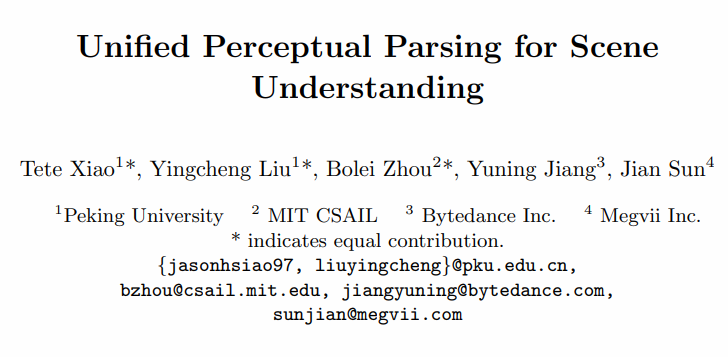
\includegraphics[width=0.9\linewidth]{Images/paper.png}
        \blfootnote{[\ref{Source1}] Xiao et al. (2018)}
        %\tiny{26 Jul 2018}
    \end{center}
\end{frame}

%-------------------------------

\begin{frame}{What is Unified Perceptual Parsing?}
    \begin{itemize}
        \item Humans perceive a scene by identifying:
        \begin{itemize}
            \item Scene type (e.g., kitchen)
            \item Objects (e.g., stove, table)
            \item Objects parts (e.g., table leg, stove knob)
            \item Materials (metal, wood)
            \item Textures (smooth, rough)
        \end{itemize}
        \item \textbf{Unified Perceptual Parsing} aims to do all this with a single model.
    \end{itemize}
    \vfill
\end{frame}

\begin{frame}{What is Unified Perceptual Parsing?}
  \begin{figure}
      \centering
        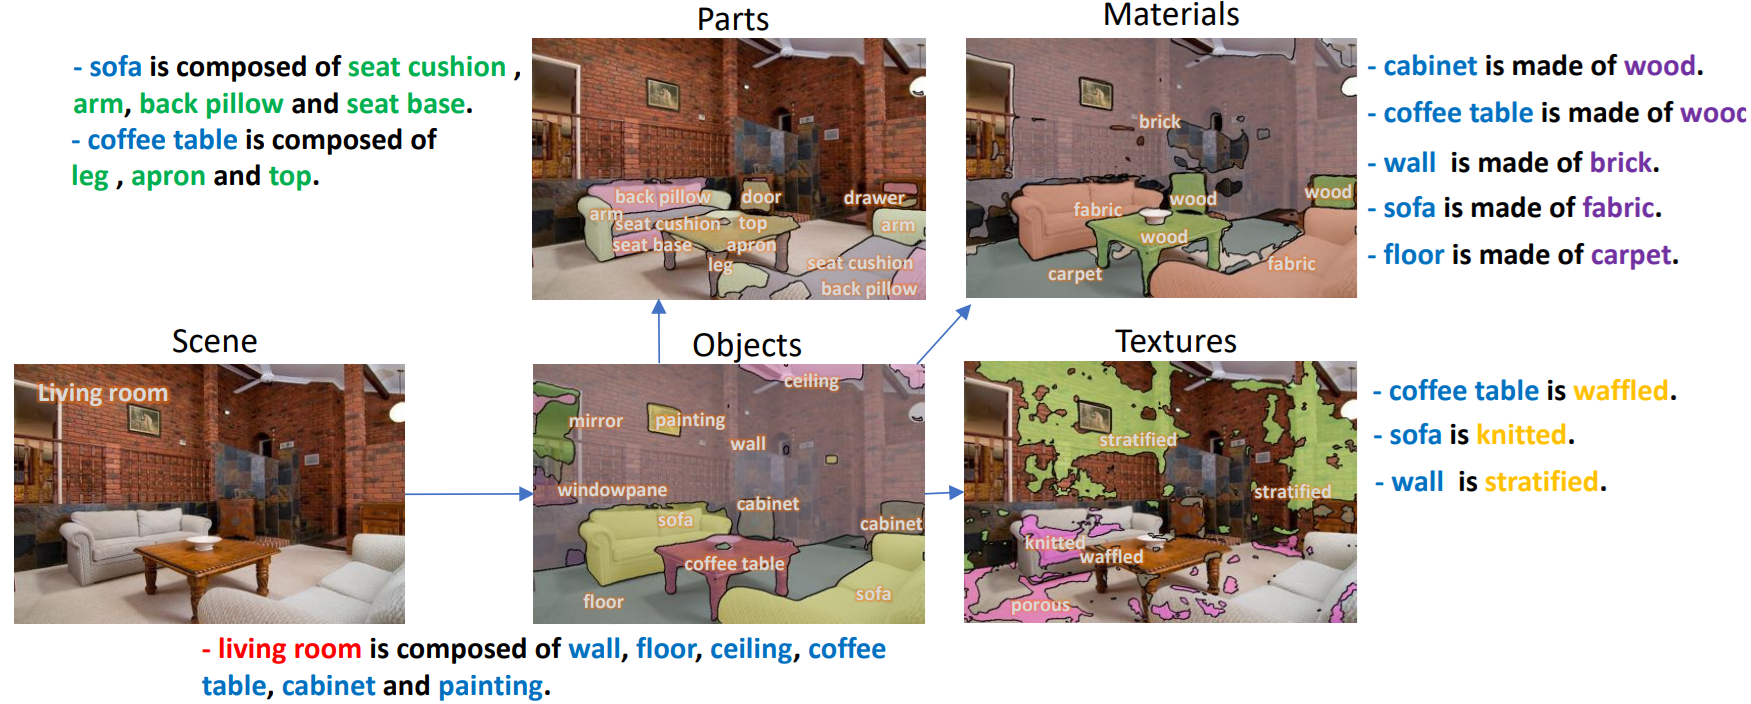
\includegraphics[width=\linewidth]{Images/intro_segmentation.png}
        \blfootnote{[\ref{Source1}] Xiao et al. (2018), Figure 1}
  \end{figure}
\end{frame}

%-------------------------------

\begin{frame}{Why Is This Challenging?}
  \begin{itemize}
    \item Perceptual parsing combines very different tasks:
    \begin{itemize}
      \item Scene classification (high-level understanding)
      \item Object and part segmentation (mid-level)
      \item Material and texture recognition (low-level, detailed)
    \end{itemize}

    \vspace{0.3cm}

    \item These tasks vary in:
    \begin{itemize}
      \item The type of information they require
      \item Spatial scale and detail level
    \end{itemize}

    \vspace{0.3cm}

    \item \textbf{Challenge:} One model must handle all levels — from big picture to fine details.
  \end{itemize}
\end{frame}

%-------------------------------

\begin{frame}{Previous Work}
  \begin{itemize}
    \item \textbf{Scene Classification:} CNNs like ResNet, trained on datasets like Places
    \item \textbf{Semantic Segmentation:} FCN, DeepLab (object-level)
    \item \textbf{Part Segmentation:} Pascal-Parts
    \item \textbf{Material / Texture:} OpenSurfaces, DTD
  \end{itemize}
  
  \begin{block}{Before This Paper:}
    \begin{itemize}
      \item Each task was handled by a separate model
      \item No feature sharing between tasks
      \item Training and inference were inefficient and fragmented
    \end{itemize}
  \end{block}
\end{frame}

%-------------------------------

\begin{frame}{Main Contribution of This Paper}
  \textbf{Objective:} Develop a single unified network for parsing multiple semantic levels from one image.

  \begin{itemize}
    \item Create \textbf{Broden+} – unified dataset from various sources
    \item Propose \textbf{UPerNet} – a multi-task network on top of FPN
    \item Define a \textbf{joint benchmark} for perceptual parsing
  \end{itemize}

  \vfill
  \textit{One image in, multiple perceptual layers out.}
\end{frame}

%-------------------------------

\begin{frame}{Why a new Dataset?}
  \textbf{No single existing dataset} had all the annotations needed for unified perceptual parsing.
  \vspace{0.4cm}

  \textbf{Limitations of existing datasets:}
  \begin{itemize}
    \item Each focuses on \textbf{only one or two tasks} (e.g., objects OR textures)
    \item Different label sets, formats, and definitions
    \item No shared vocabulary across datasets (e.g. 'car' in one dataset might be 'vehicle' in another)
  \end{itemize}
  \vfill
  \textit{Manual merging needed to create a unified dataset that supports all tasks.}
\end{frame}

\begin{frame}{How Was Broden+ Merged?}
  
  \textbf{Merging Criteria:}
  \begin{itemize}
    \item All annotations are \textbf{mapped to a shared vocabulary}
    \item Images are labeled with \textbf{as many tasks as possible}
    \item Only high-quality, pixel-aligned annotations are kept
    \item Some rare classes were \textbf{merged into broader categories} to reduce noise and improve consistency (e.g 'stone' and 'concrete' are merged into 'stone')
  \end{itemize}
\end{frame}

\begin{frame}{What is Broden+}
  \begin{itemize}
    \item \textbf{Broden+} is a large-scale, unified dataset built by merging:
    \begin{itemize}
      \item ADE20K: Scene and object segmentation
      \item Pascal-Context: Part segmentation
      \item OpenSurfaces: Material labels
      \item DTD (Describable Textures Dataset): Texture attributes
    \end{itemize}
    \item Provides a \textbf{diverse set of annotations} per image:
    \begin{itemize}
      \item Scene labels, object masks, parts, textures, materials
    \end{itemize}
  \end{itemize}
\end{frame}

%-------------------------------

\begin{frame}{UPerNet Architecture Overview}
    \begin{figure}
        \centering
        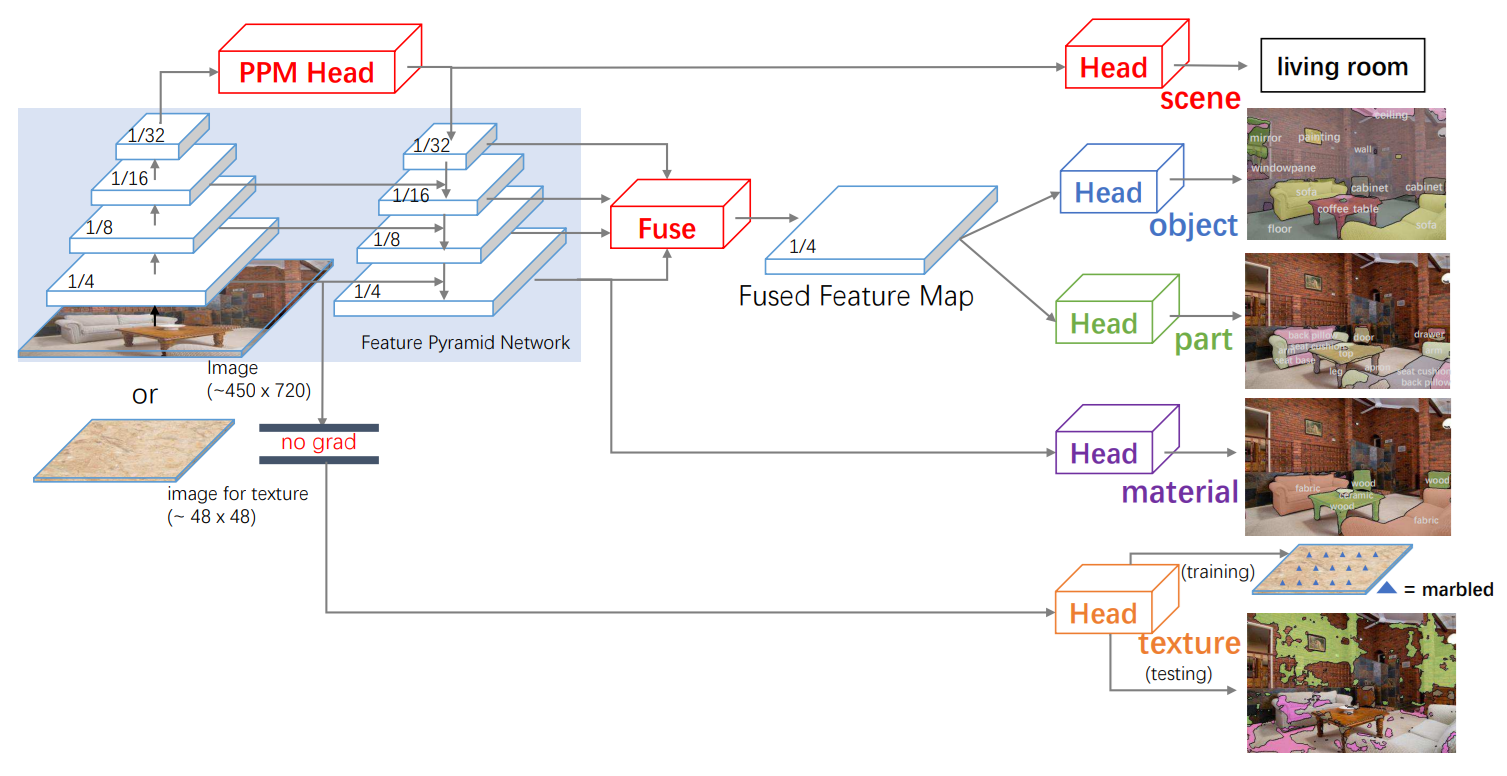
\includegraphics[width=\textwidth]{Images/UPerNetArchitectureOverview_noHeads.png}
        \blfootnote{[\ref{Source1}] Xiao et al. (2018), Figure 4 (edited)}
    \end{figure}
\end{frame}

%-------------------------------

\begin{frame}{Feature Pyramid Networks (FPN)}
    \begin{figure}
        \centering
        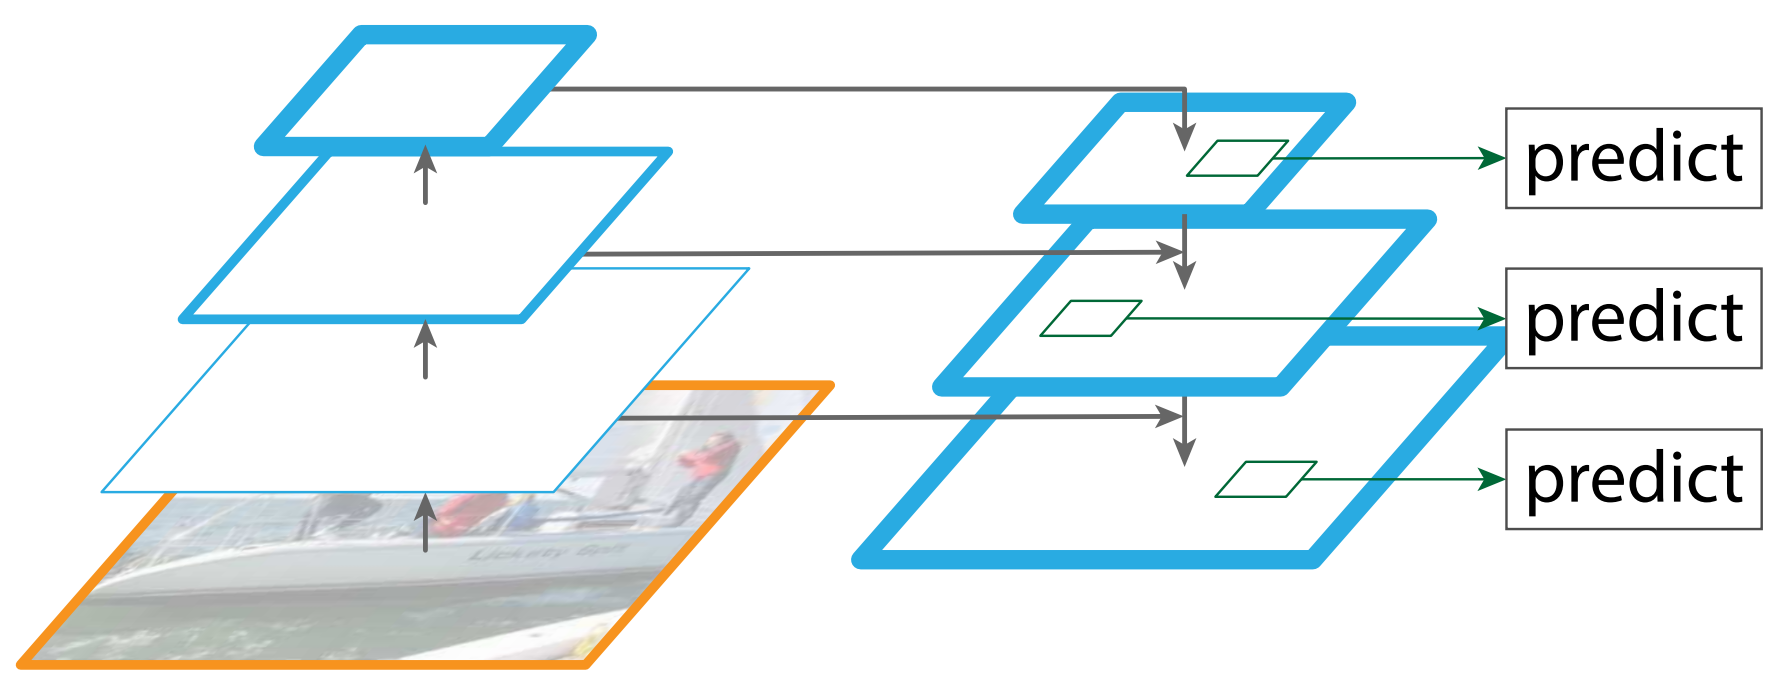
\includegraphics[width=0.7\textwidth]{Images/FPNOverview.png}
        \blfootnote{[\ref{Source2}] Lin et al. (2017), Figure 1 (edited)}
    \end{figure}
    \vspace{-0.5 cm}
    \begin{itemize}
        \item \textbf{Bottom-up pathway:} Computes feature maps at different scales using a convolutional NN
        \item \textbf{Top-down pathway:} Upsamples high-level feature maps back to original size (nearest neighbour upsampling)
        \item \textbf{Lateral connections:} Merges feature maps of \textbf{Top-down pathway} with \textbf{Bottom-up pathway} from same level in hierarchy
    \end{itemize}
\end{frame}

%-------------------------------

\begin{frame}{UPerNet Architecture Overview}
    \begin{figure}
        \centering
        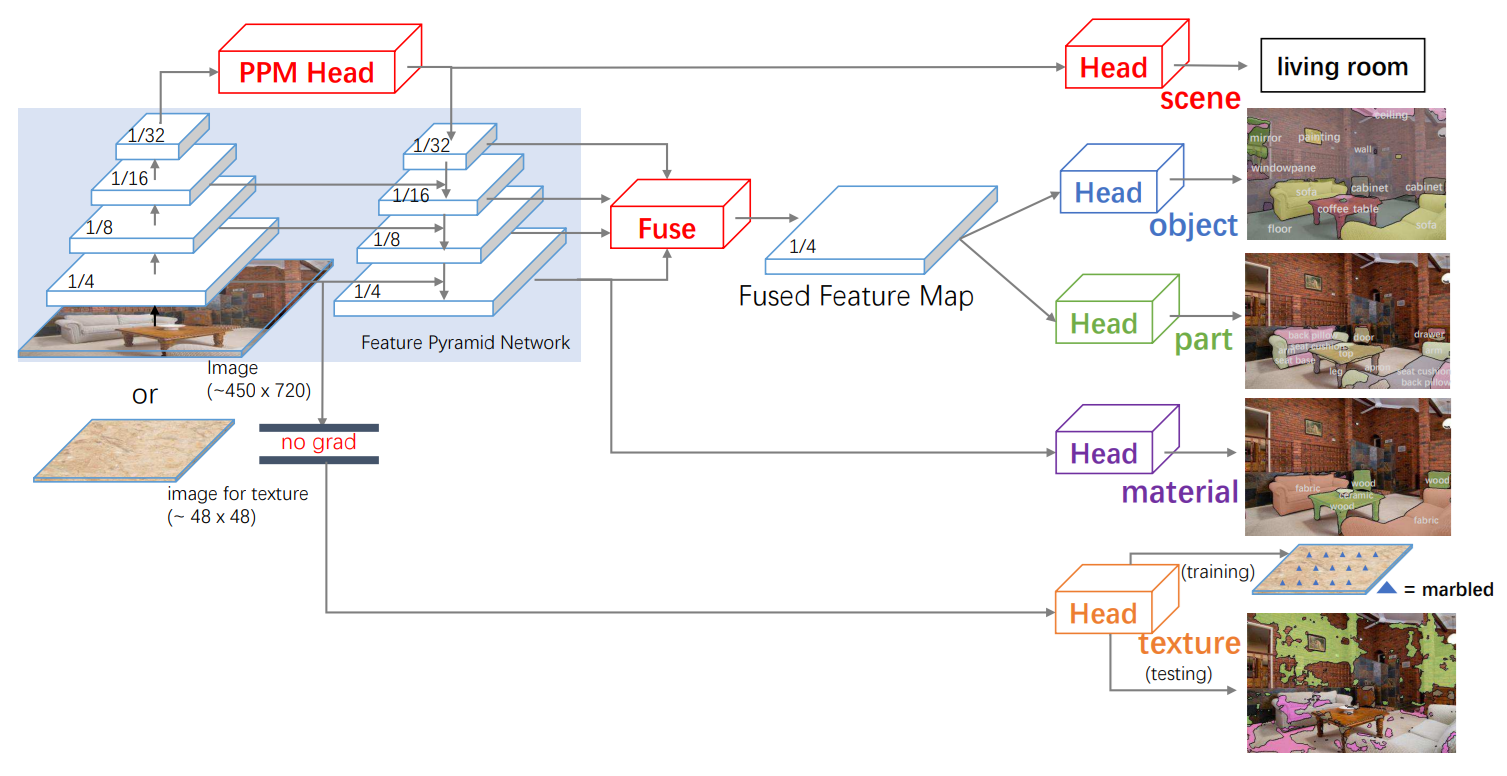
\includegraphics[width=\textwidth]{Images/UPerNetArchitectureOverview_noHeads.png}
        \blfootnote{[\ref{Source1}] Xiao et al. (2018), Figure 4 (edited)}
    \end{figure}
\end{frame}

%-------------------------------

\begin{frame}{Pyramid Pooling Module}
    \begin{figure}
        \centering
        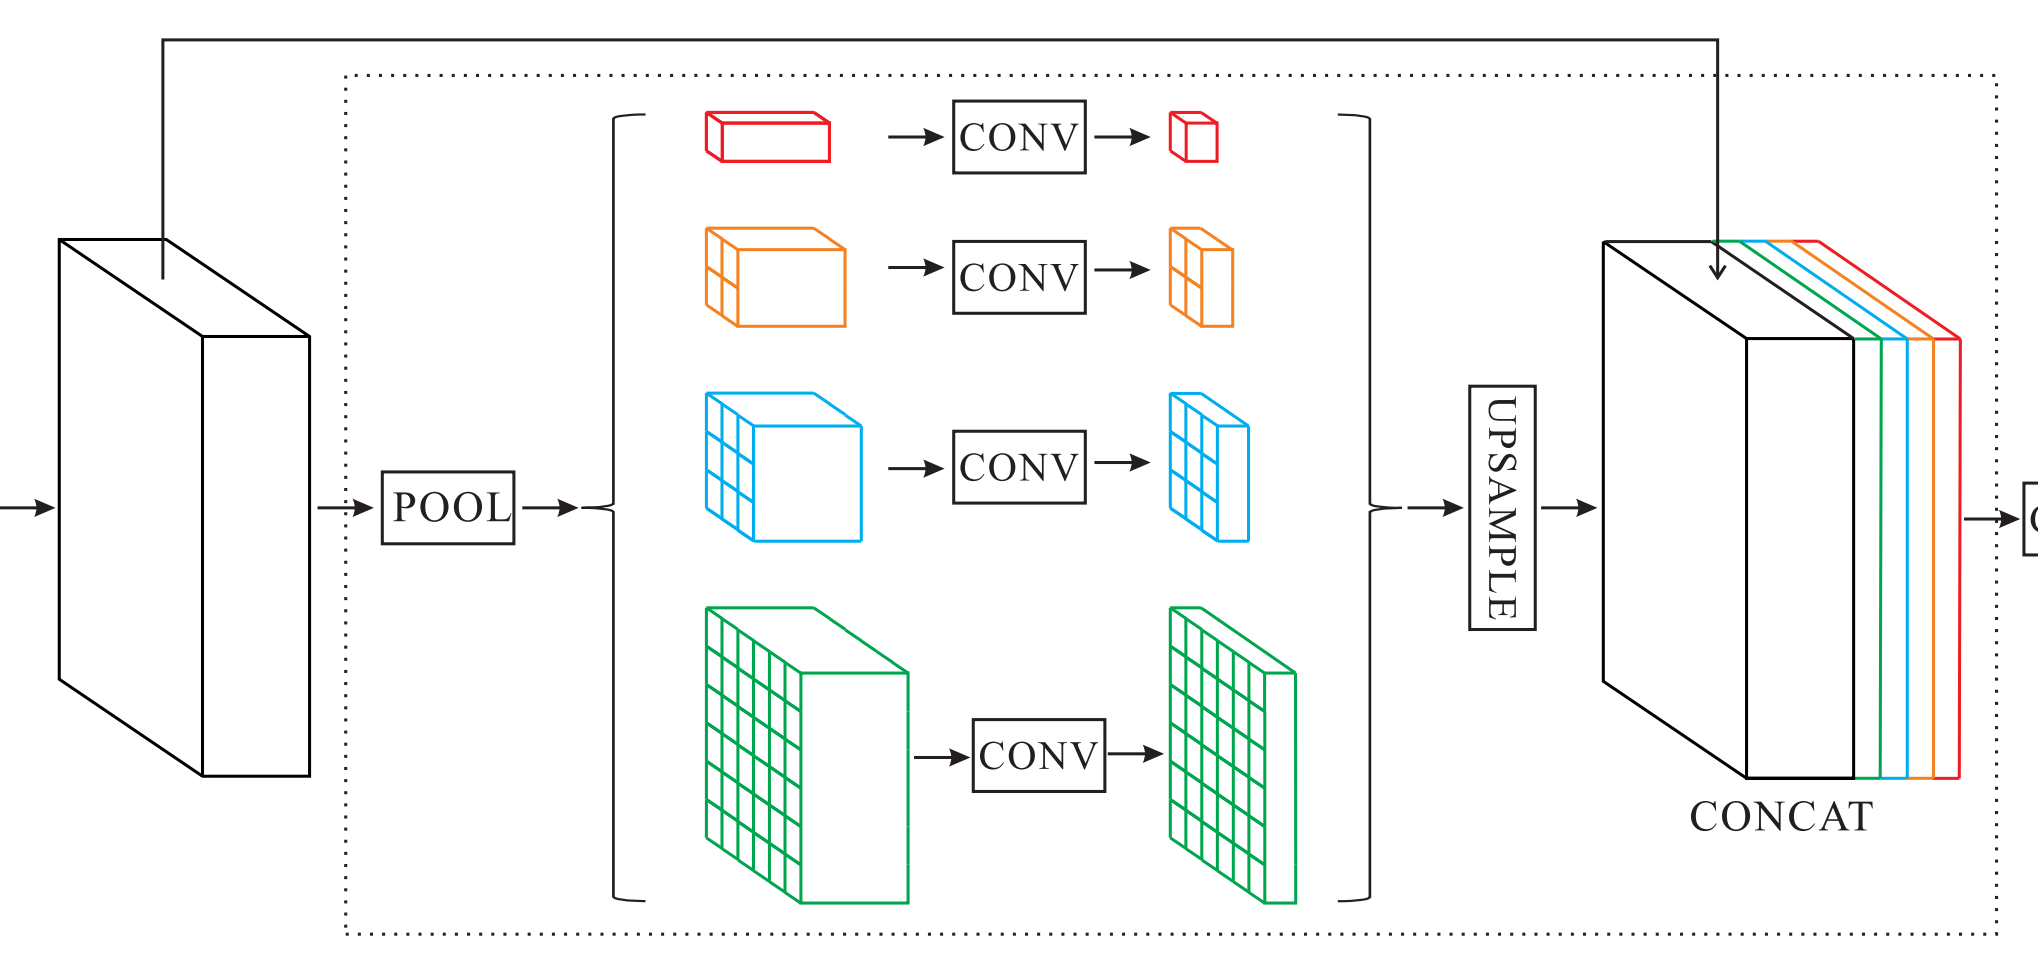
\includegraphics[width=0.7\textwidth]{Images/PPMModuleOverview.png}
        \blfootnote{[\ref{Source3}] Zhao et al. (2017), Figure 3 (edited)}
    \end{figure}
    \vspace{-0.5cm}
    \begin{itemize}
        %\item Input is a feature map provided by some CNN
        \item Different pooling operations produce different sized feature maps
        \item Reduce dimensionality with a 1x1 convolution
        \item Upsample via interpolation to original size
        \item Concatenate results with original feature map
        \item PPM is used to address limited receptive field of deep CNNs
    \end{itemize}
\end{frame}

%-------------------------------

\begin{frame}{UPerNet Architecture Overview}
    \begin{figure}
        \centering
        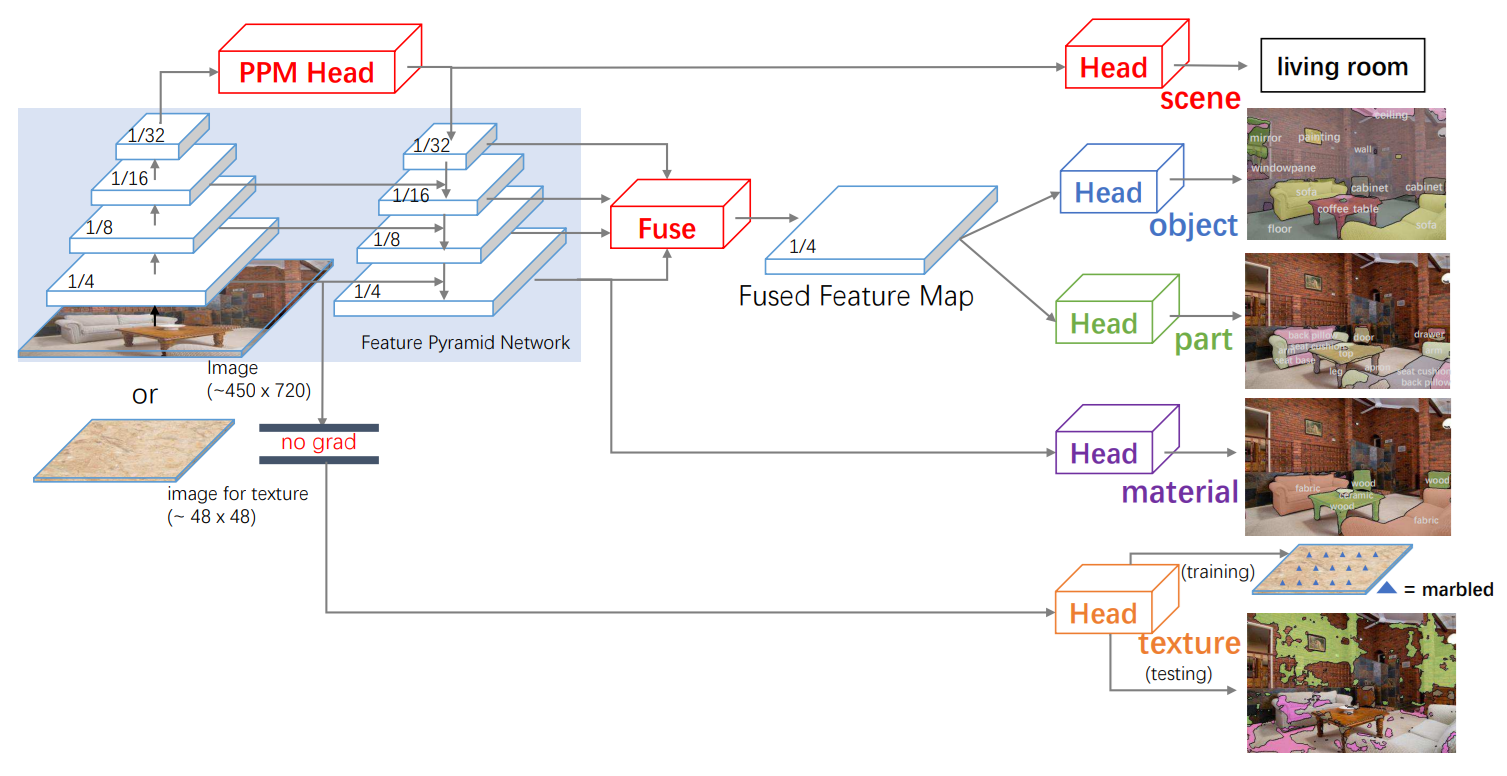
\includegraphics[width=\textwidth]{Images/UPerNetArchitectureOverview_noHeads.png}
        \blfootnote{[\ref{Source1}] Xiao et al. (2018), Figure 4 (edited)}
    \end{figure}
\end{frame}

%-------------------------------

\begin{frame}{Classification Heads}
    \begin{figure}
        \centering
        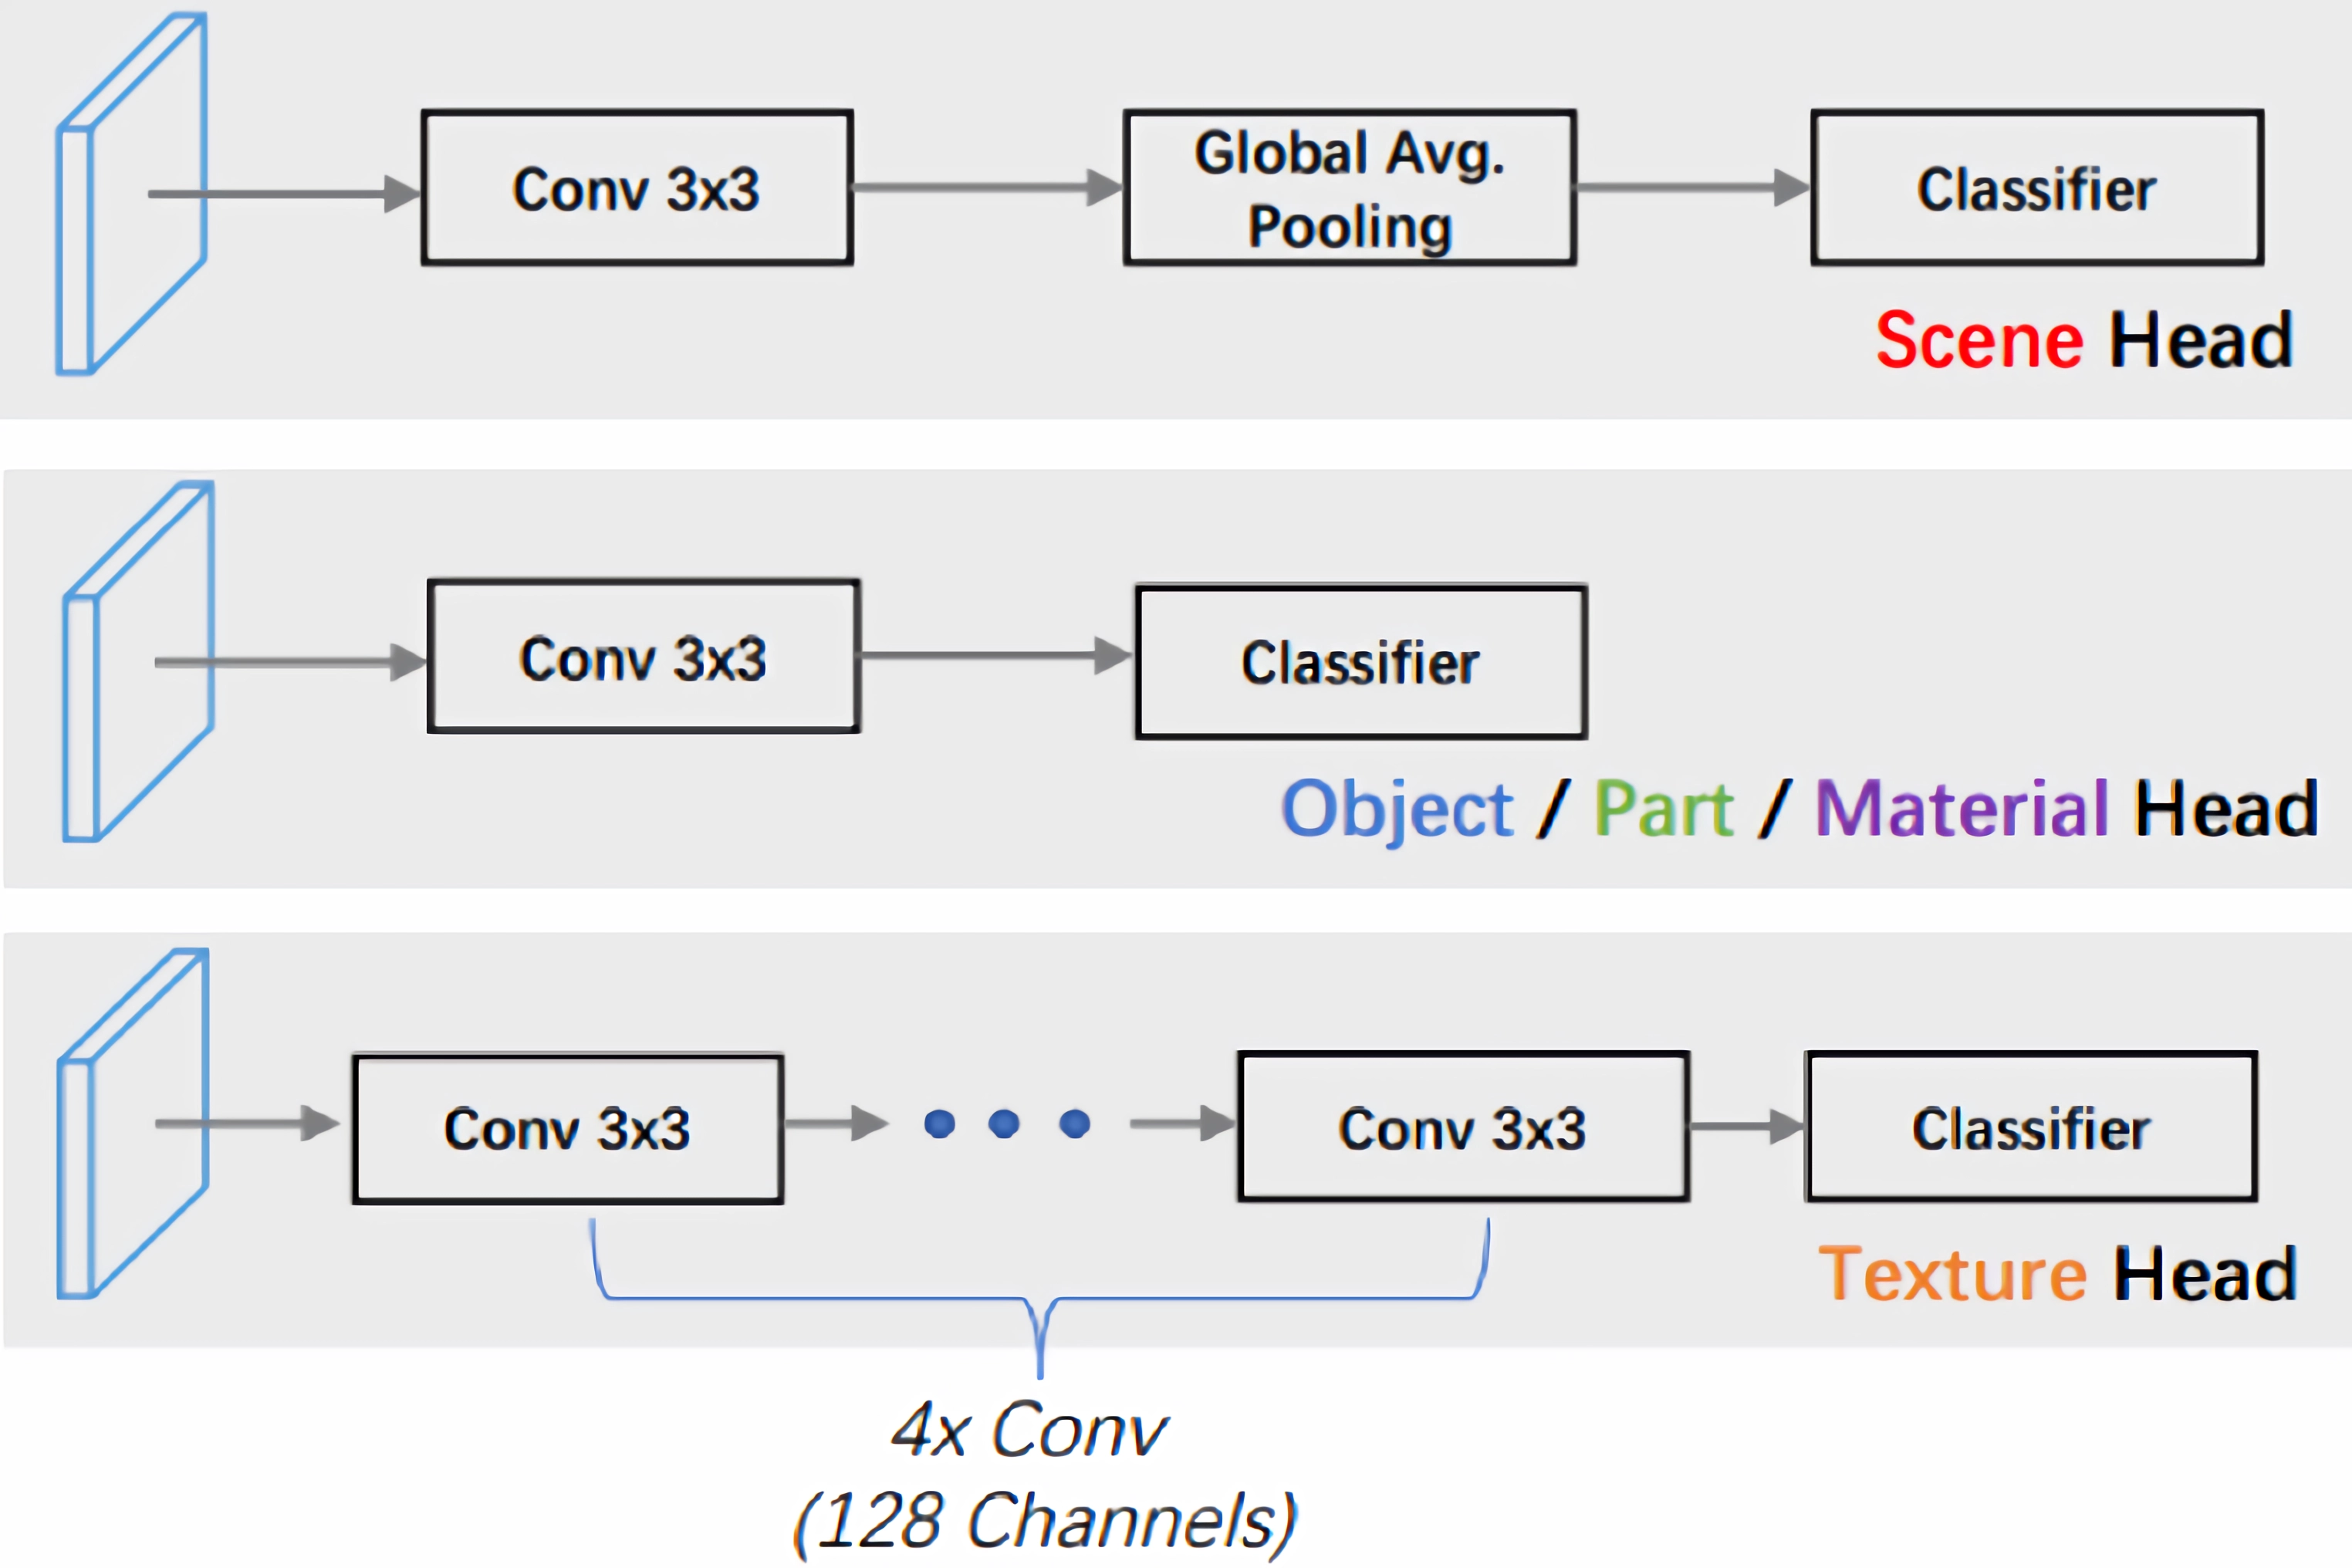
\includegraphics[width=0.7\textwidth]{Images/ClassifierHeads.png}
        \blfootnote{[\ref{Source1}] Xiao et al. (2018), Figure 4 (edited)}
    \end{figure}
\end{frame}


%-------------------------------

\begin{frame}{Experiment 1: Standard Semantic Segmentation}
  Comparison with state-of-the-art methods for semantic segmentation of objects on the ADE20K dataset:
  \begin{figure}
    \centering
    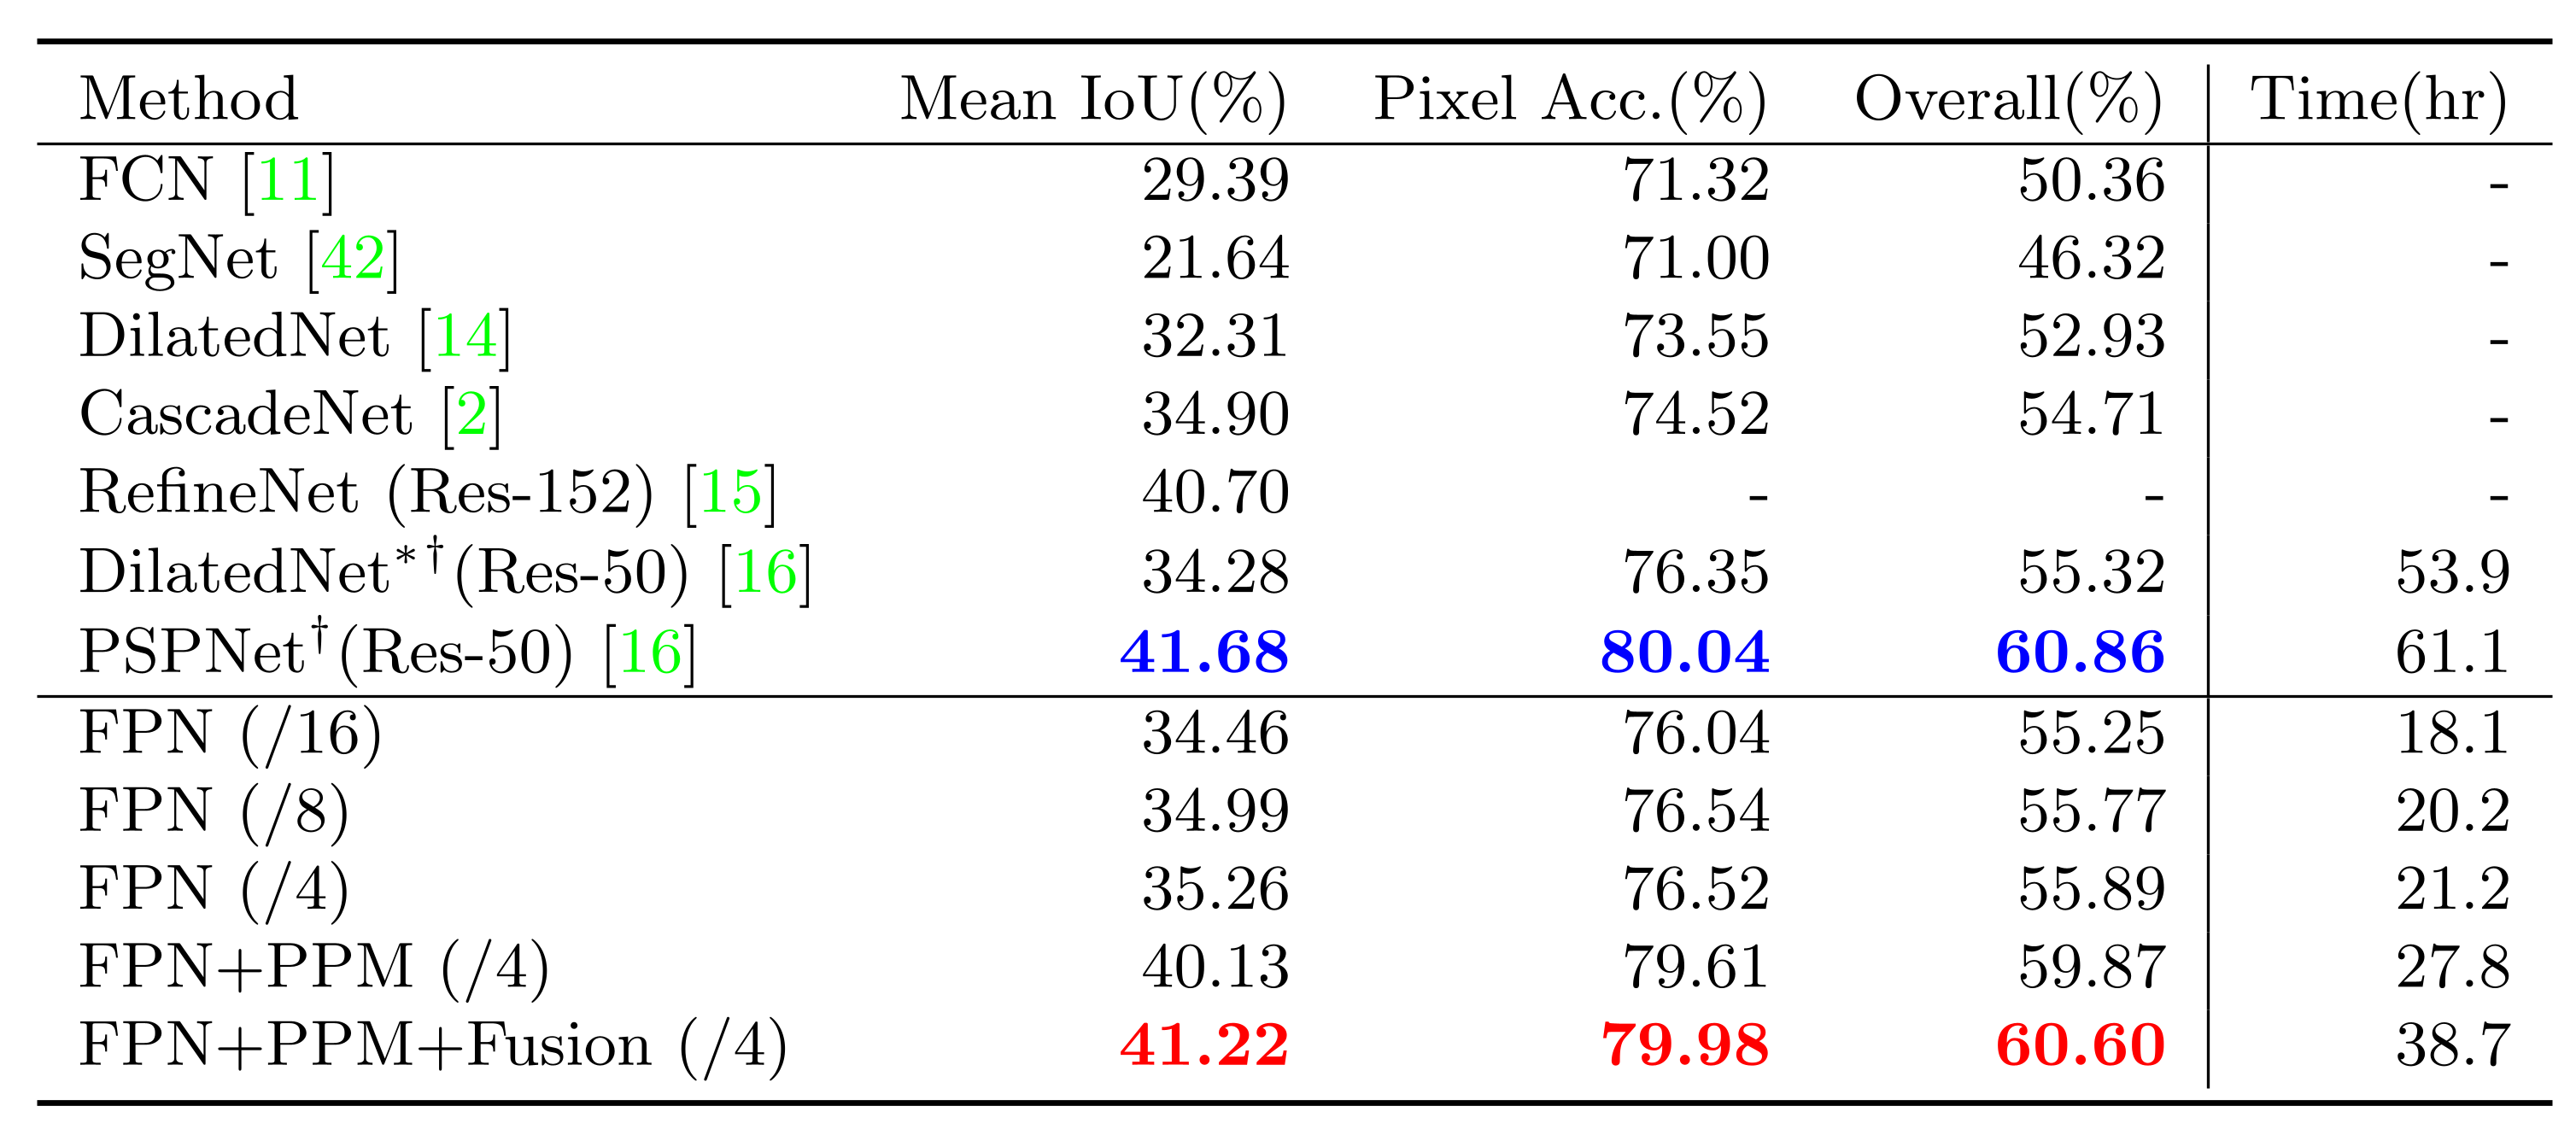
\includegraphics[width=\textwidth]{Images/Table2.png}
    \blfootnote{[\ref{Source1}] Xiao et al. (2018), Table 2}
  \end{figure}
\end{frame}

%    \item Was heißt "\emph{Our results are obtained without multi-scale inference or other techniques.}"?

\begin{frame}{Experiment 2: Unified Perceptual Parsing}
  Results of UPP on the Broden+ dataset:
  \begin{figure}
    \centering
    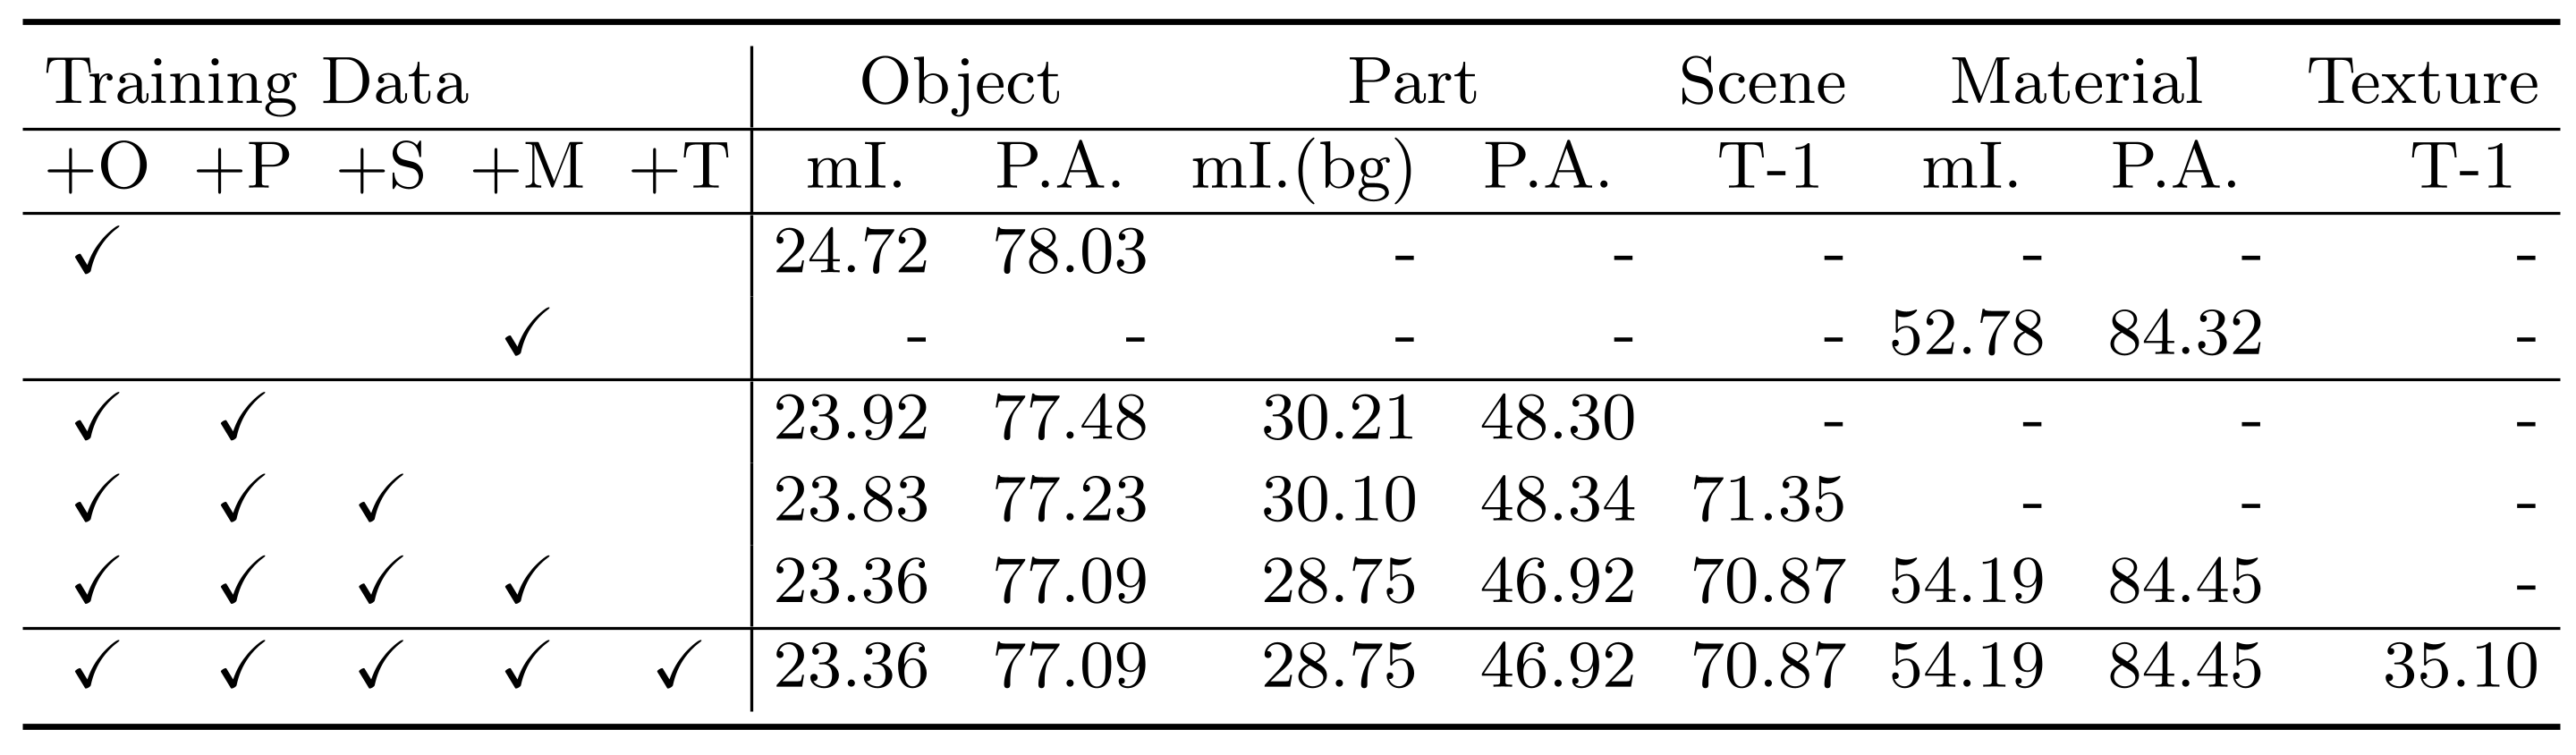
\includegraphics[width=\textwidth]{Images/Table3.png}
    \blfootnote{[\ref{Source1}] Xiao et al. (2018), Table 3}
  \end{figure}
  \vspace{-1cm}
  \begin{itemize}
    \item Joint training across 5 perceptual levels
    \item Performance remains stable for most tasks and even improves for material
    \item Texture prediction requires fine-tuning due to different data distribution
  \end{itemize}
\end{frame}

\begin{frame}{Experiment 2: Unified Perceptual Parsing}
  Some qualitative results:
  \vspace{-0.25cm}
  \begin{figure}
    \centering
    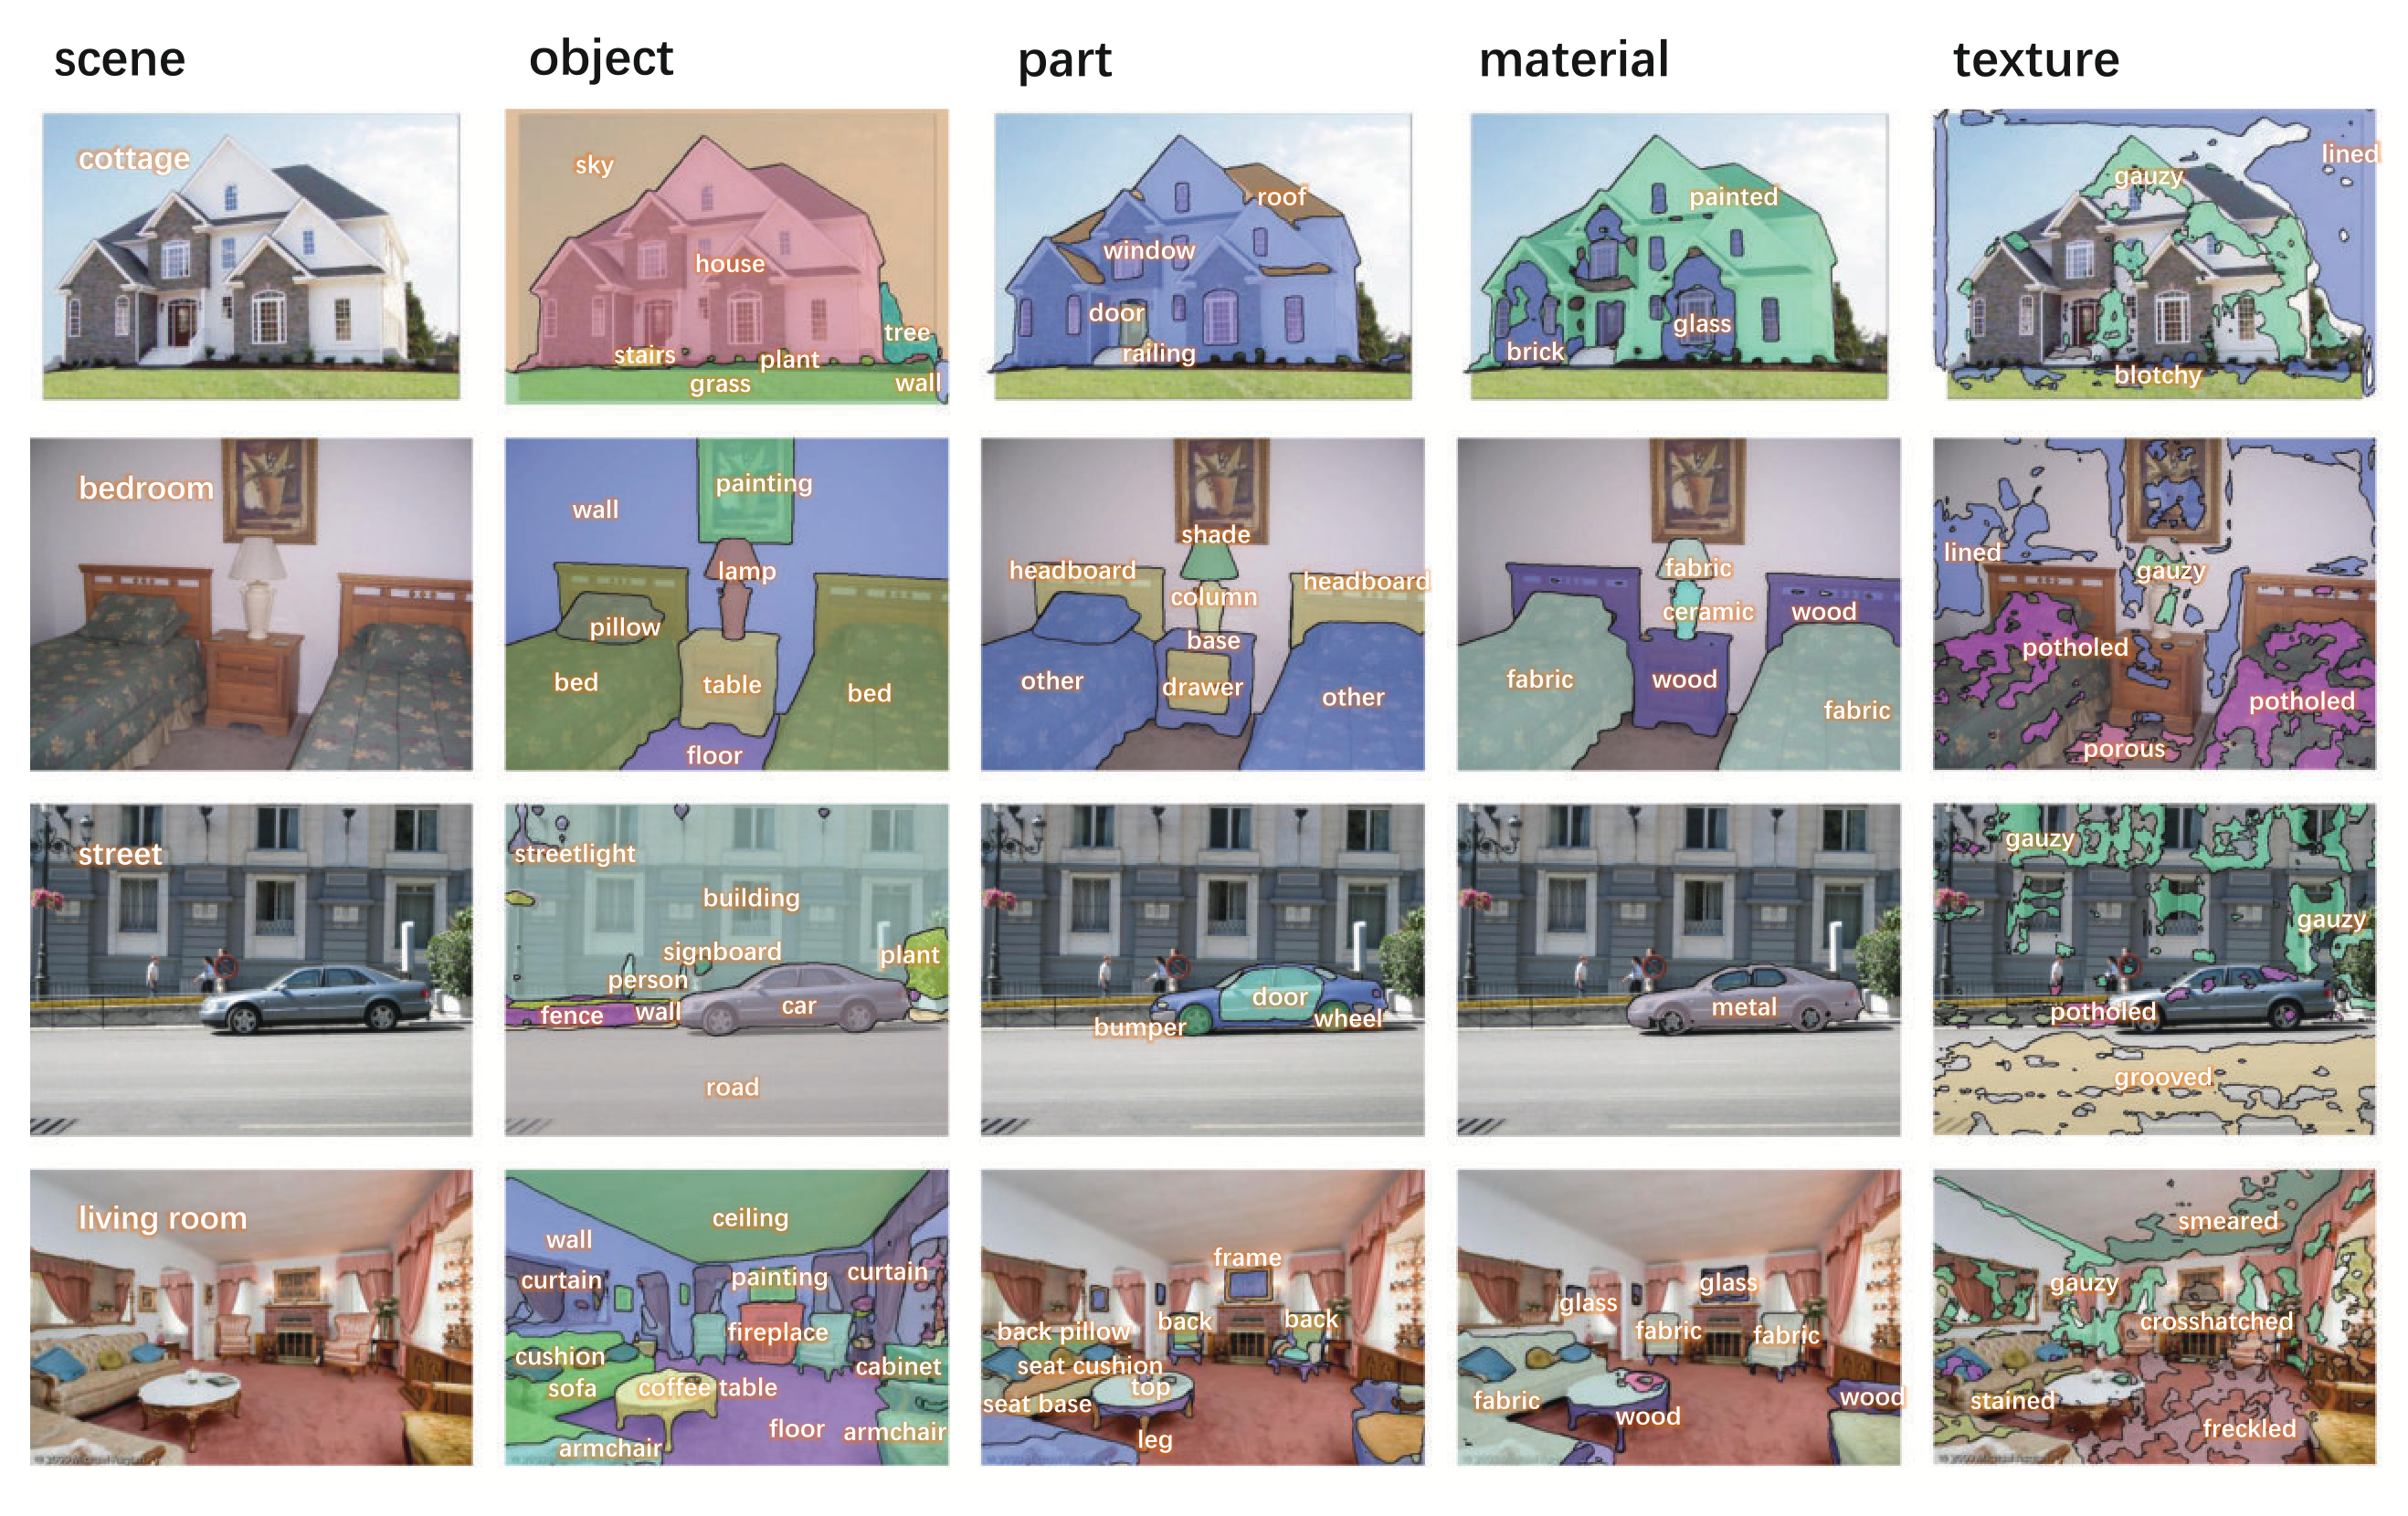
\includegraphics[width=\textwidth]{Images/Figure5 Springer.png}
    \blfootnote{[\ref{Source1}] Xiao et al. (2018), Figure 5}
  \end{figure}
  \vspace{-1cm}
\end{frame}

\begin{frame}{Visual Knowledge Discovery}
  Visualization of scene-object relations after clustering:
  \vspace{-0.25cm}
  \begin{figure}
    \centering
    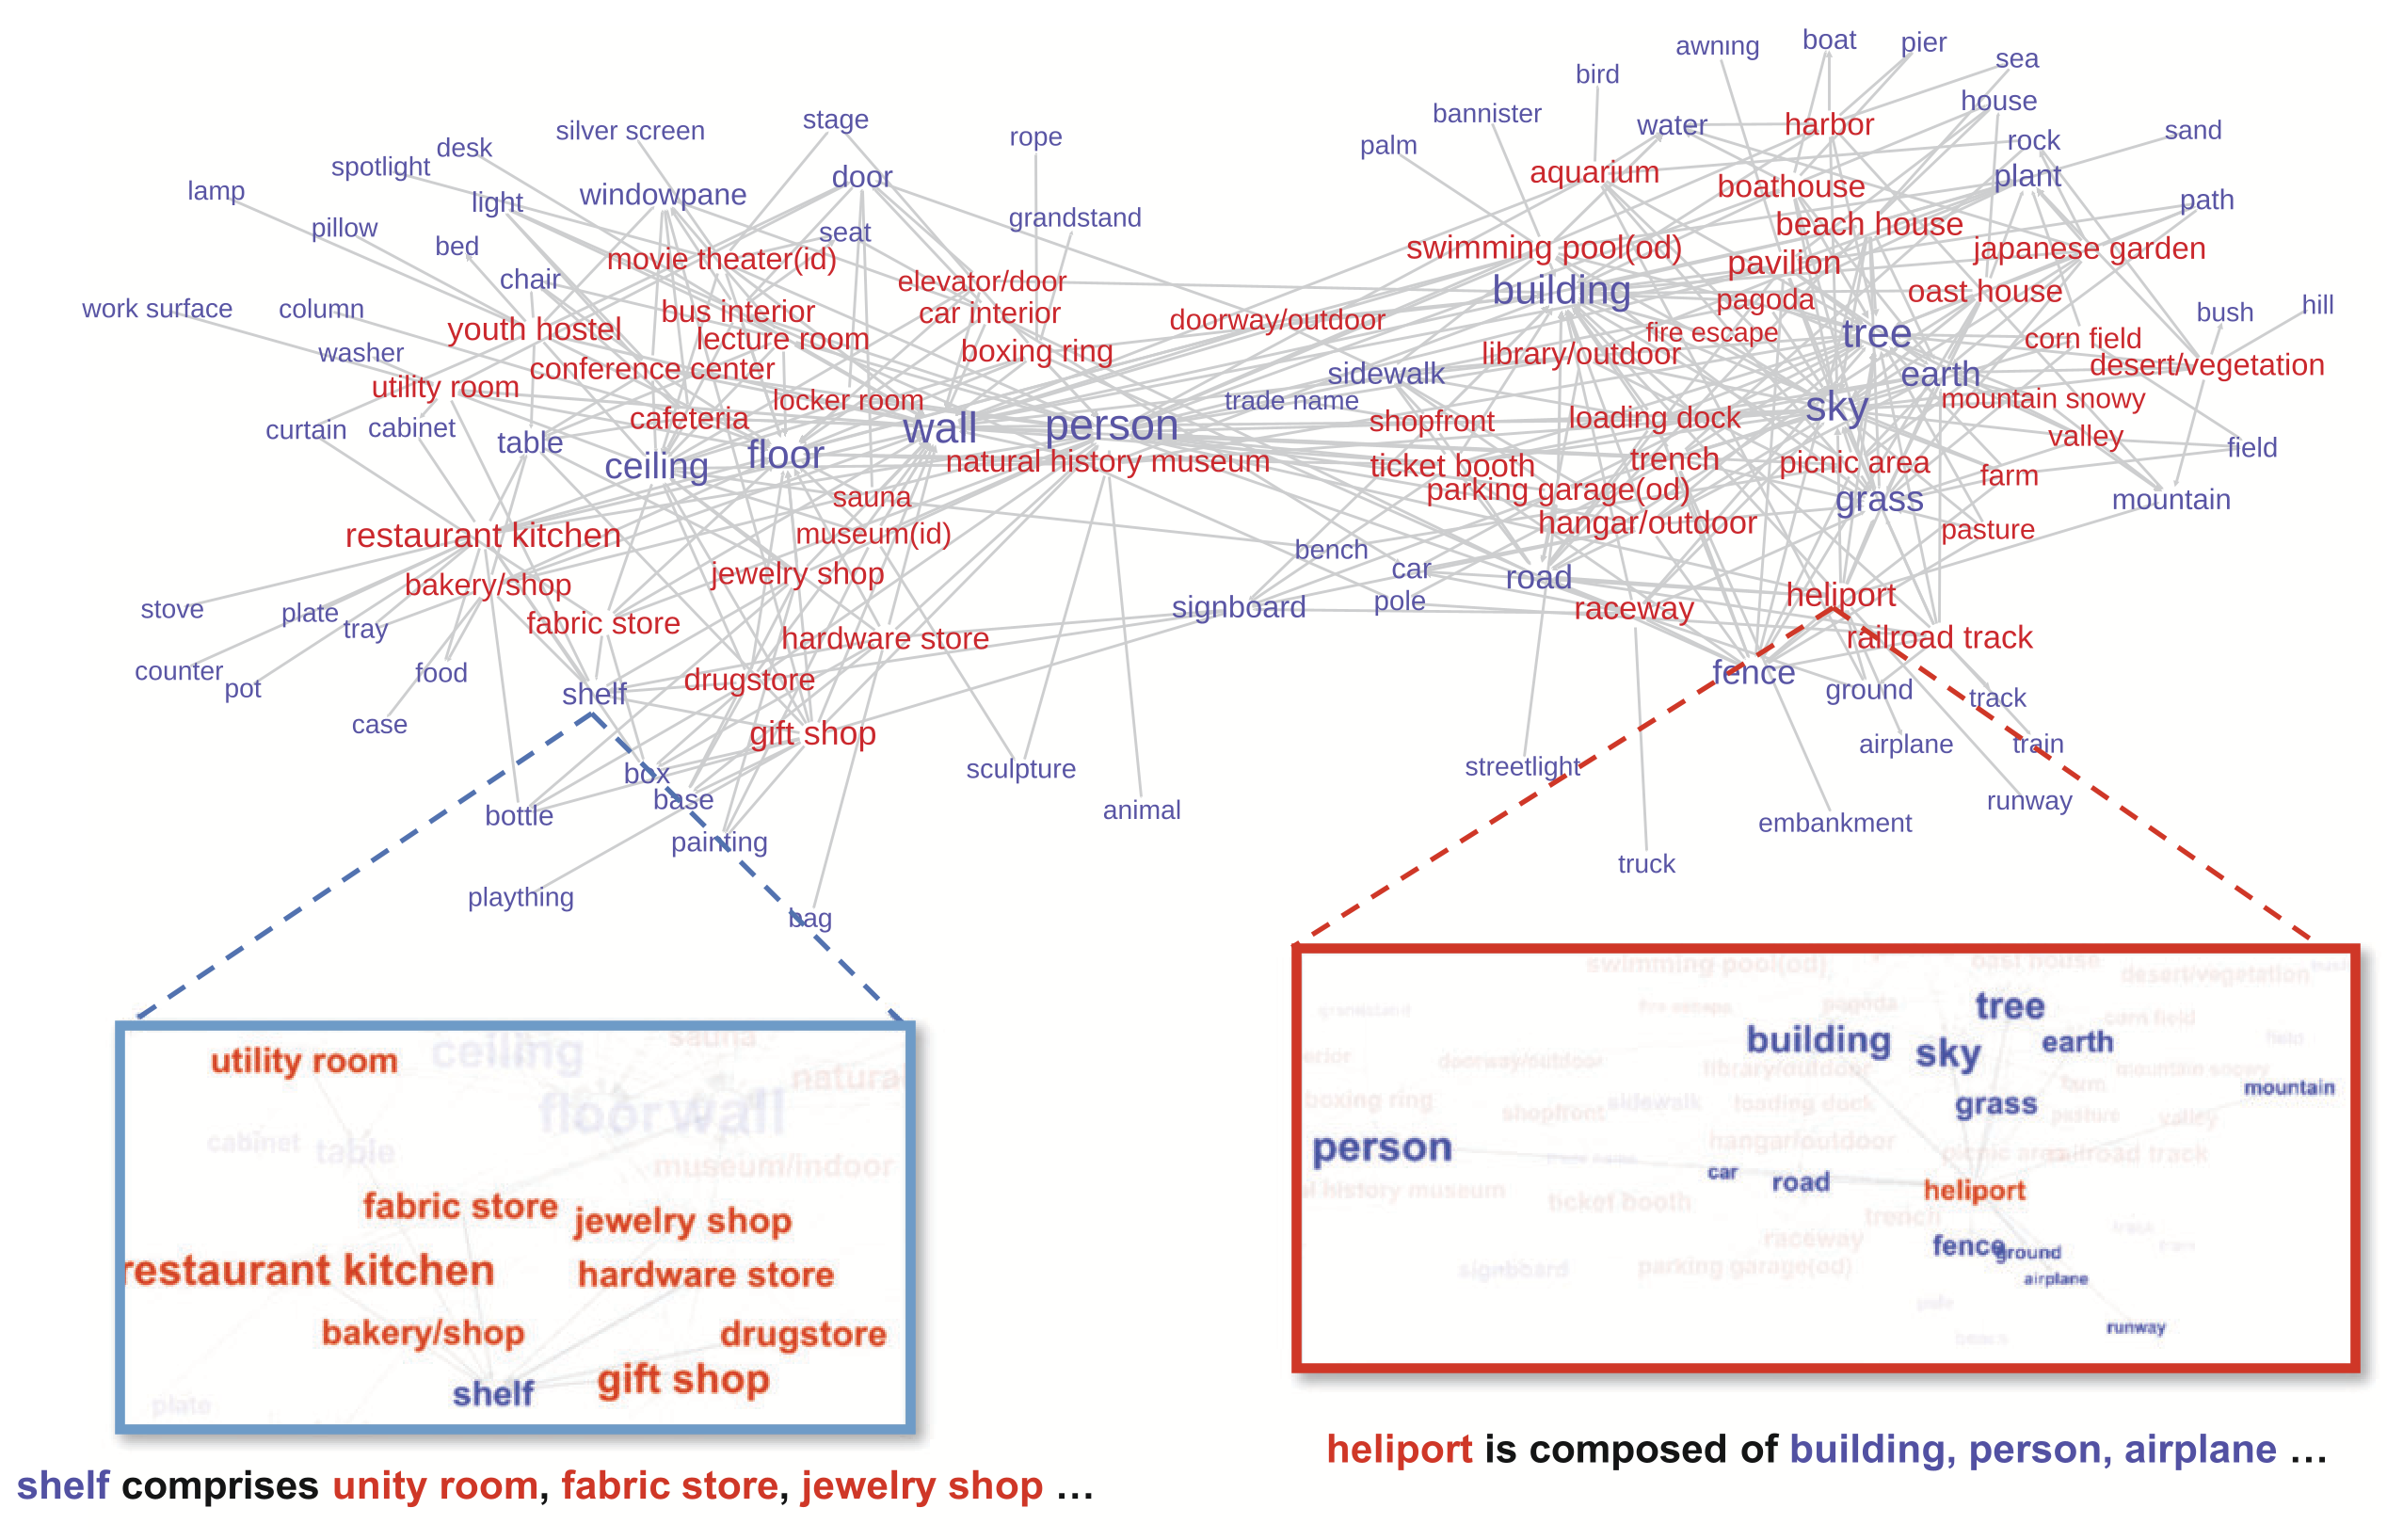
\includegraphics[width=\textwidth]{Images/Figure6a.png}
    \blfootnote{[\ref{Source1}] Xiao et al. (2018), Figure 6a}
  \end{figure}
  \vspace{-1cm}
\end{frame}

\begin{frame}{Visual Knowledge Discovery}
  \begin{figure}
    \centering
    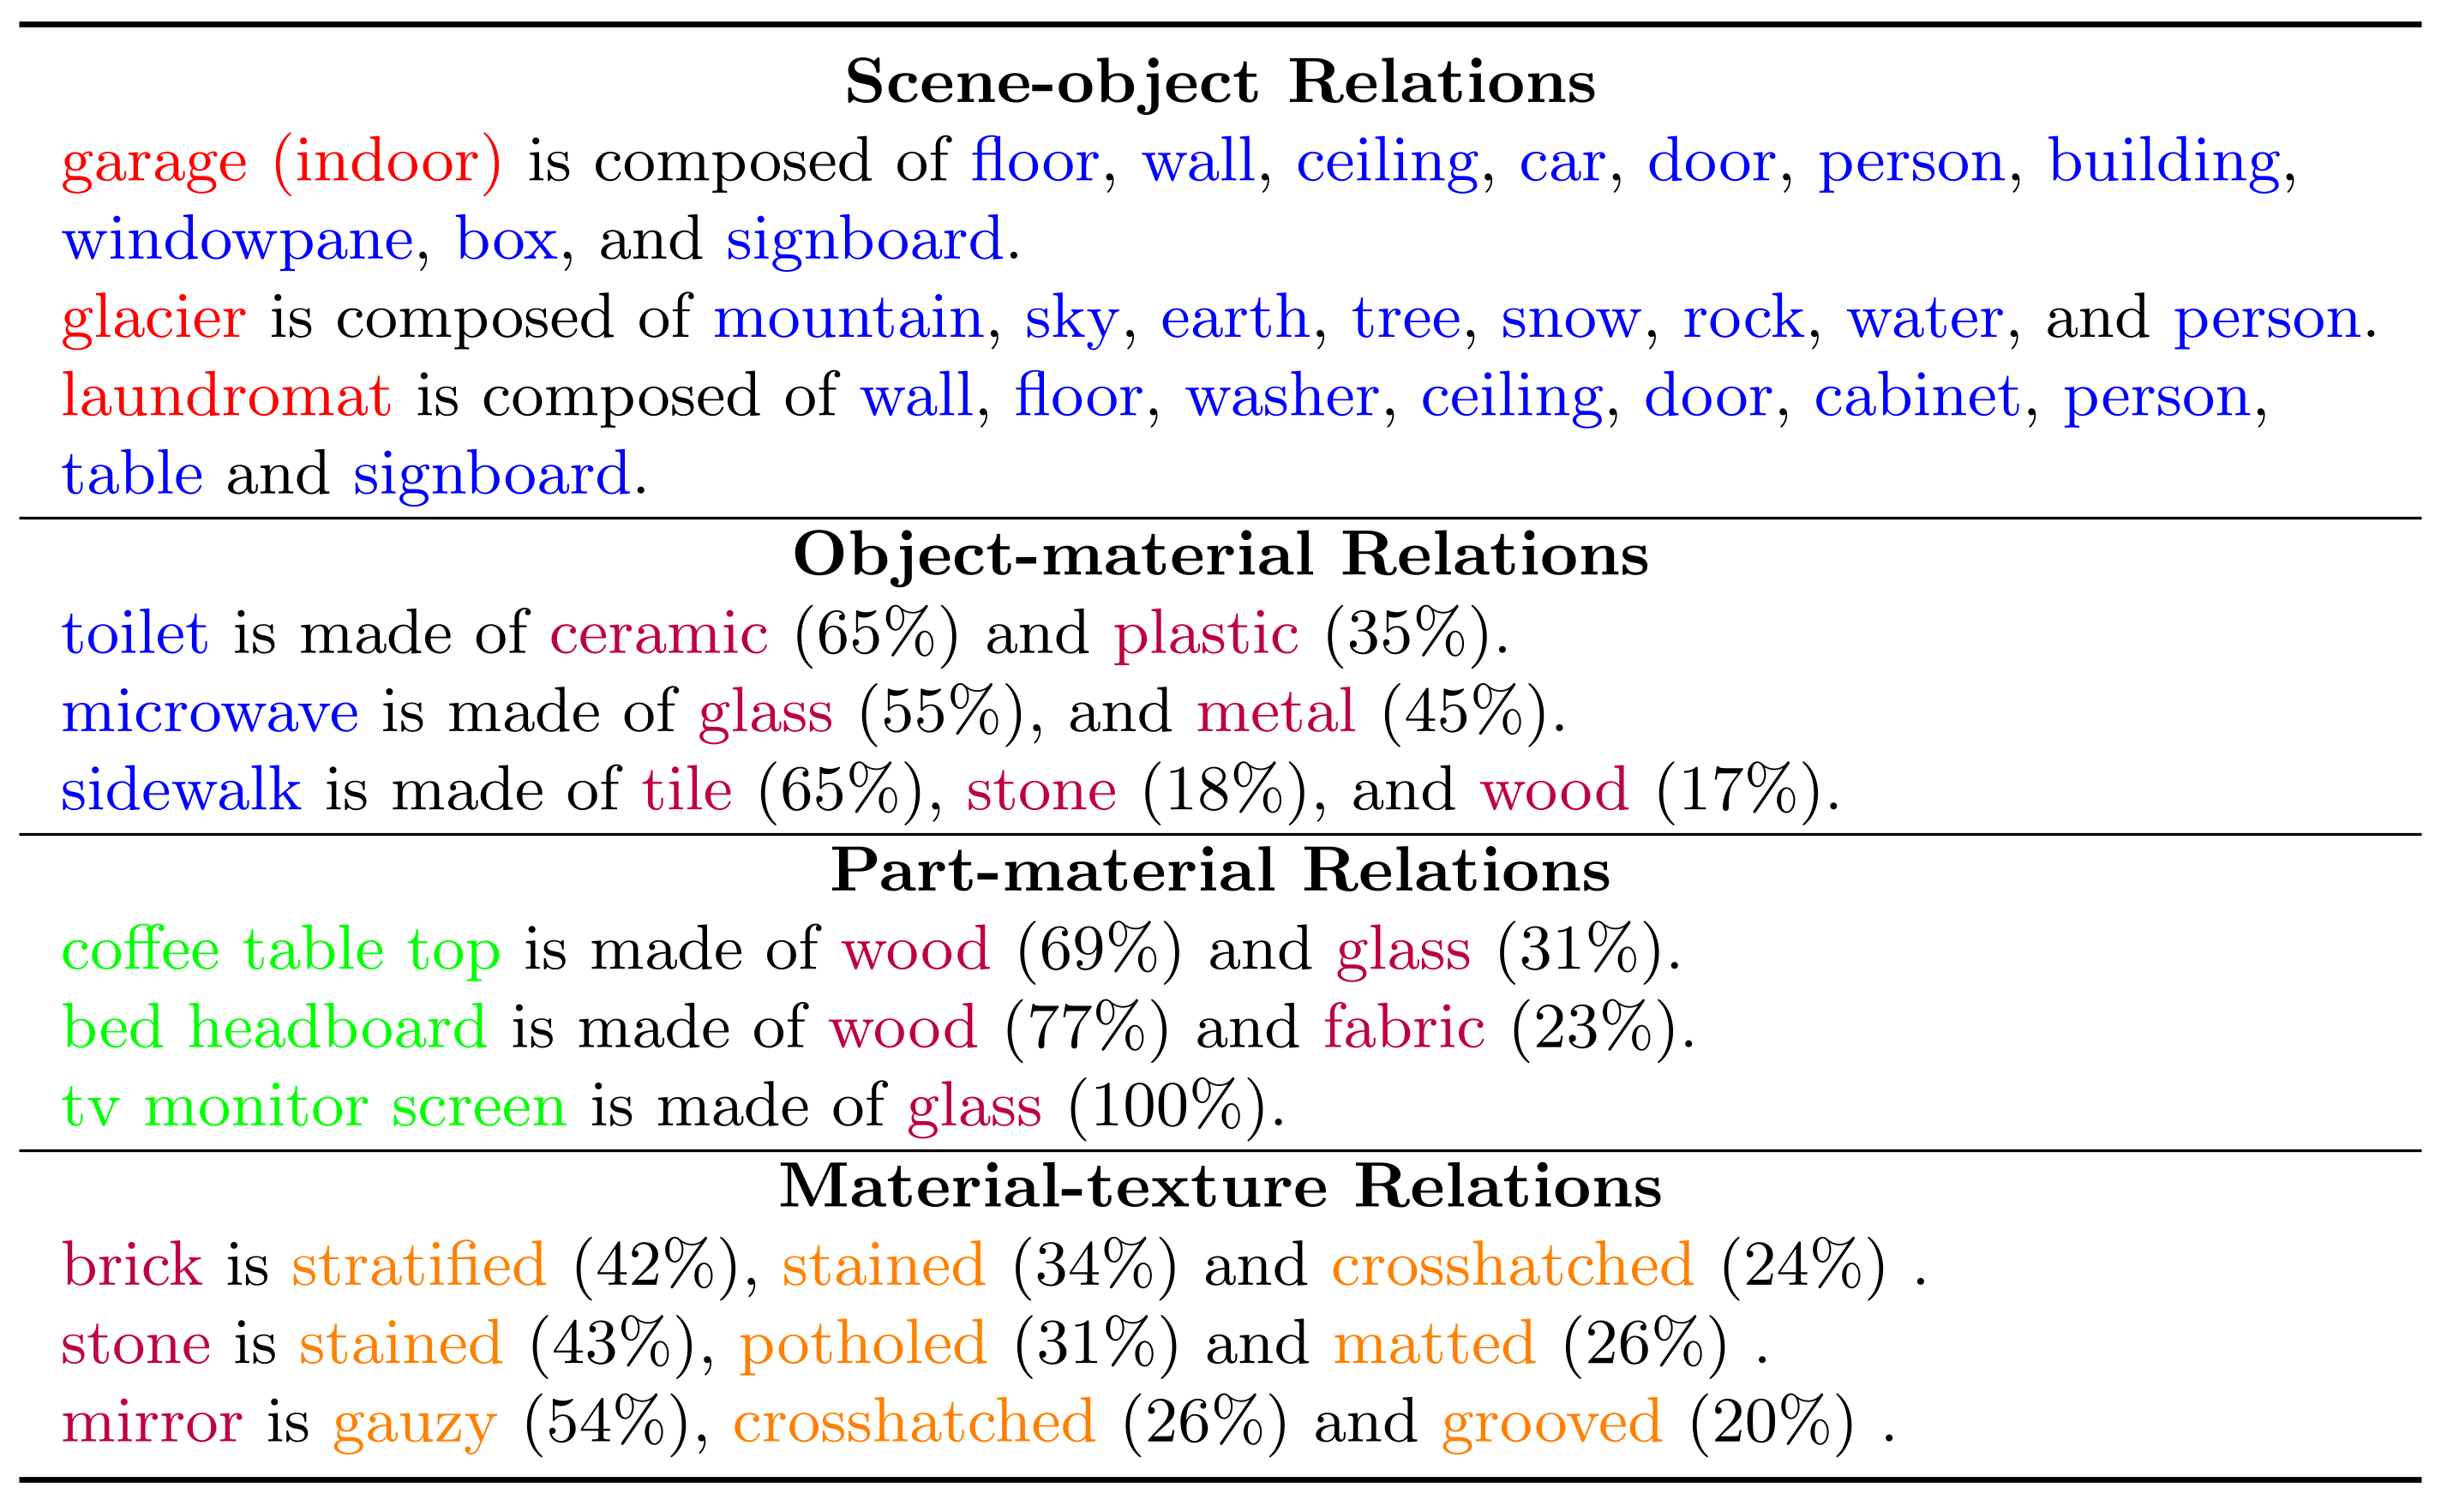
\includegraphics[width=\textwidth]{Images/Table4.png}
    \blfootnote{[\ref{Source1}] Xiao et al. (2018), Table 4}
  \end{figure}
\end{frame}

% Slide 4 – Conclusion and Perspective
\begin{frame}{Conclusion and Perspectives}
  \begin{itemize}
    \item UPerNet performs competitively on semantic segmentation with less training time
    \item The network can handle heterogeneous annotations and tasks across multiple perception levels
    \item Allows for discovery of compositional visual knowledge (e.g. scene-object-material relations)
    \item Future directions:
    \begin{itemize}
      \item Improving texture parsing and handling more complex real-world images
      \item Potential for downstream applications in robotics, AR and reasoning
    \end{itemize}
  \end{itemize}
\end{frame}

% Slide 5 – Open Questions
\begin{frame}{Open Questions}
\begin{figure}
    \centering
    
\includegraphics[height=0.8\textheight]{Images/Questions.jpg}
\end{figure}
\end{frame}

\appendix
\setbeamertemplate{navigation symbols}{}

\begin{frame}{Literature}
\small
\begin{enumerate}[ {[}1{]} ]
    \item \label{Source1} T. Xiao et al., ``Unified Perceptual Parsing for Scene Understanding'' in \emph{Computer Vision – ECCV 2018: 15th European Conference, Munich, Germany, September 8–14, 2018, Proceedings, Part V}, 2018, pp. 432–448, doi: \href{https://doi.org/10.1007/978-3-030-01228-1_26}{10.1007/978-3-030-01228-1\_26}.
    
    \item \label{Source2} T.-Y. Lin et al., ``Feature Pyramid Networks for Object Detection'' in \emph{2017 IEEE Conference on Computer Vision and Pattern Recognition (CVPR)}, 2017, pp. 936–944, doi: \href{https://doi.org/10.1109/CVPR.2017.106}{10.1109/CVPR.2017.106}.
    
    \item \label{Source3} H. Zhao et al., ``Pyramid Scene Parsing Network'' in \emph{2017 IEEE Conference on Computer Vision and Pattern Recognition (CVPR)}, 2017, pp. 6230–6239, doi: \href{https://doi.org/10.1109/CVPR.2017.660}{10.1109/CVPR.2017.660}.
\end{enumerate}
\end{frame}

\section{Backup}

\begin{frame}{How Was Broden+ Merged?}
\centering
  \begin{figure}
    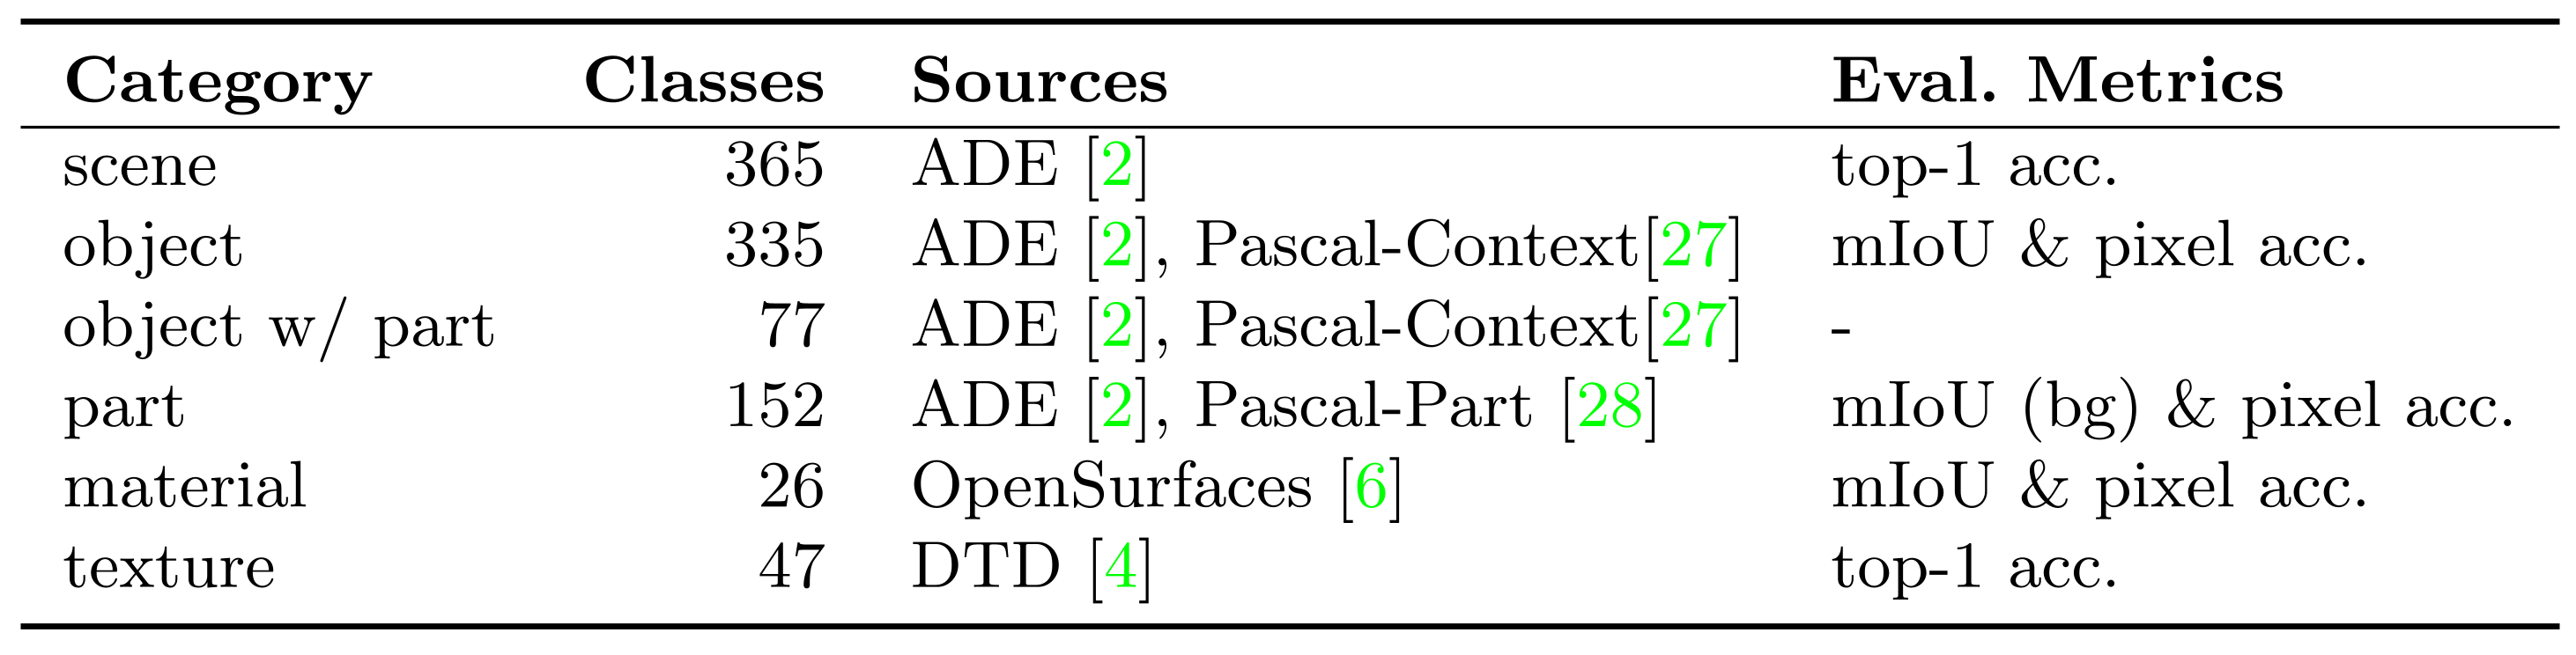
\includegraphics[width=\linewidth]{Images/Table1.png}
  \end{figure}
  \begin{figure}
    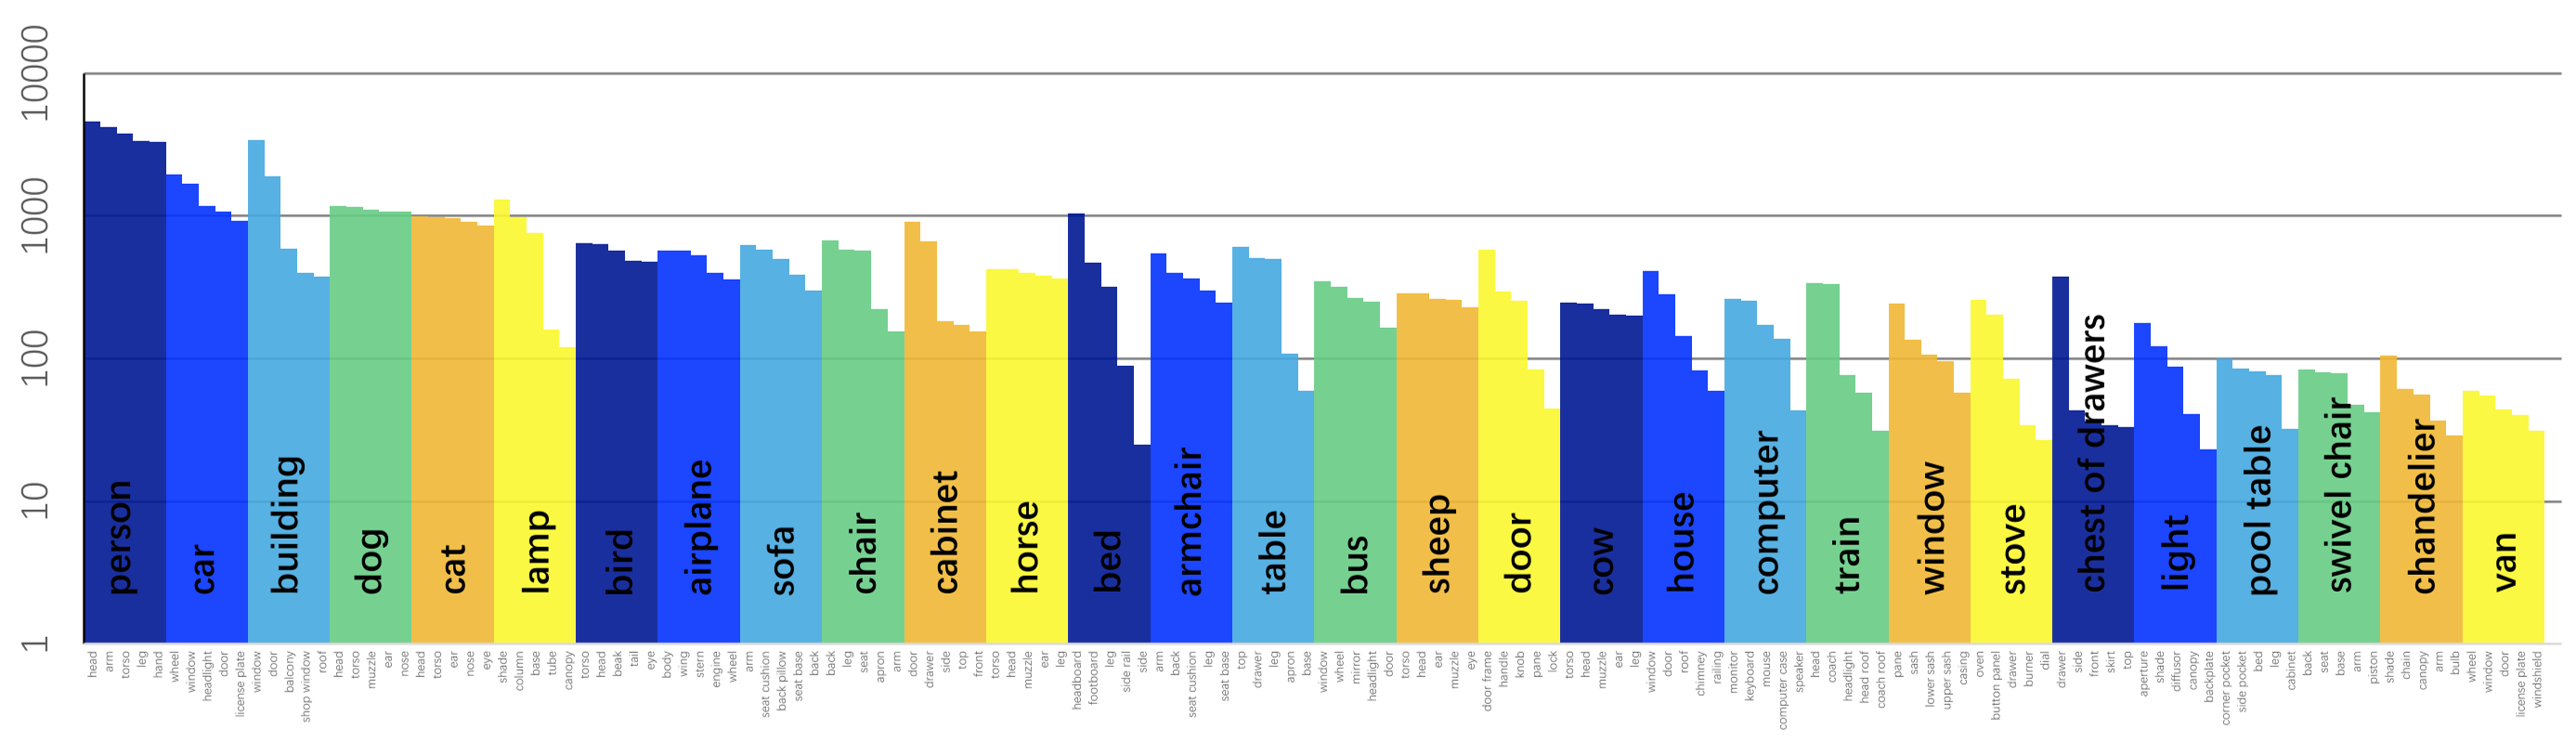
\includegraphics[width=\linewidth]{Images/Figure 2b.png}
    \blfootnote{[\ref{Source1}] Xiao et al. (2018), Table 1 + Figure 2b}
  \end{figure}
\end{frame}

%-------------------------------

\begin{frame}{How Is Performance Measured?}
  \vspace{0.4cm}
  \begin{tabular}{ll}
    \textbf{Task} & \textbf{Metric} \\
    \hline
    Scene Classification & Top-1 Accuracy \\
    Object Segmentation & Mean IoU (Intersection over Union) \\
    Part Segmentation & Mean IoU \\
    Material Prediction & Pixel Accuracy \\
    Texture Prediction & Image-level Classification Accuracy \\
  \end{tabular}
  \vspace{0.5cm}
  \begin{itemize}
    \item Evaluated on the unified benchmark created from \textbf{Broden+}.
    \item \textbf{Multi-task setting:} All tasks evaluated using a shared backbone and features.
  \end{itemize}
  \vfill
  \textit{Goal: Assess how well the unified model performs across diverse visual tasks.}
\end{frame}

\end{document}